\documentclass[12pt]{article}

%------------------------------------------------------------------------------
%	Preparation	
%------------------------------------------------------------------------------

% packages and macros
\usepackage[utf8]{inputenc}
\usepackage[english]{babel}
\usepackage[titletoc]{appendix}
\usepackage{sjlatex/stata}
\usepackage{float}

\usepackage[nottoc,notlot,notlof]{tocbibind}
\usepackage{bbm}
\usepackage{xifthen}
\usepackage{amsmath}
\usepackage{amsfonts}
\usepackage{natbib}
\usepackage{amsthm}
\usepackage{appendix}
\usepackage[ruled,vlined]{algorithm2e}
\usepackage{graphicx}
\usepackage{epstopdf}

\usepackage{geometry}
\setlength{\headheight}{14pt}
\setlength{\topmargin}{0pt}
\setlength{\textheight}{620pt}
\setlength{\footskip}{10pt}
\setlength{\oddsidemargin}{0pt}
\setlength{\evensidemargin}{0pt}
\geometry{
  top=15mm,
  left=15mm,
}

\usepackage{hyperref}
\hypersetup{
colorlinks,
citecolor=black,
filecolor=black,
linkcolor=black,
urlcolor=black
}


\usepackage{setspace}
\onehalfspacing

\usepackage{enumitem}

\newtheorem{defi}{DEFINITION}
\newtheorem{lemma}{LEMMA}
\newtheorem{assumption}{ASSUMPTION}
\newtheorem{theorem}{THEOREM}
\newtheorem{remark}{REMARK}
\newtheorem{prop}{PROPOSITION}

\newcommand{\ivqreg}{{\tt ivqregress}}
\newcommand{\ivqregiqr}{{\tt ivqregress iqr}}
\newcommand{\ivqregsee}{{\tt ivqregress smooth}}
\newcommand{\I}{\mathbbm{1}}
\newcommand{\Is}{\widetilde{\mathbbm{1}}}
\newcommand{\E}{\mathbf{E}}
\newcommand{\hsee}{h^*_{SEE}}
\DeclareMathOperator*{\argmax}{arg\,max}
\DeclareMathOperator*{\argmin}{arg\,min}

\newcommand{\Xb}{\mathbf{X}}
\newcommand{\Db}{\mathbf{D}}
\newcommand{\Zb}{\mathbf{Z}}
\newcommand{\UD}{U_\Db}
\newcommand{\Wb}{\mathbf{W}}
\newcommand{\xb}{\mathbf{x}}
\newcommand{\db}{\mathbf{d}}
\newcommand{\zb}{\mathbf{z}}
\newcommand{\Ud}{U_\db}
\newcommand{\Yd}{Y_\db}
\newcommand{\bb}{\mathbf{b}}
\newcommand{\Jb}{\mathbf{J}}
\newcommand{\Sb}{\mathbf{S}}
\newcommand{\Ab}{\mathbf{A}}
\newcommand{\Rb}{\mathbf{R}}
\newcommand{\rb}{\mathbf{r}}
\newcommand{\vb}{\mathbf{v}}
\newcommand{\gb}{\mathbf{g}}
\newcommand{\cb}{\mathbf{c}}
\newcommand{\gammab}{\boldsymbol{\gamma}}
\newcommand{\betab}{\boldsymbol{\beta}}
\newcommand{\alphab}{\boldsymbol{\alpha}}
\newcommand{\thetab}{\boldsymbol{\theta}}
\newcommand{\Psib}{\boldsymbol{\Psi}}
\newcommand{\Phib}{\boldsymbol{\Phi}}
\newcommand{\Omegab}{\boldsymbol{\Omega}}
\newcommand{\Lambdab}{\boldsymbol{\Lambda}}


\newcommand{\dil}[1]{{\color{red}#1}}


% title
\title{\ivqreg: Stata Command for Instrumental Variables Quantile Regression}
\author{Di Liu \\ StataCorp}
\date{March 31, 2022}

\begin{document}
\titlepage
\maketitle

%------------------------------------------------------------------------------
%	Head
%------------------------------------------------------------------------------

% abstract
%------------------------------------------------------------------------------
%	abstract
%------------------------------------------------------------------------------
\begin{abstract}
We describe the design of {\ivqreg}, a Stata command to estimate the linear
quantile regression model with endogenous variables using the instrumental
variables approach.  In particular, {\ivqreg} implements the inverse quantile
regression estimator in \cite{Chernozhukov2006} and the smoothed estimating
equation estimator in \cite{Kaplan2017}.  We also give details about the design
of a suite of post-estimation tools to visualize, make inference, and diagnose
the instrumental variable quantile regression model. 
\end{abstract}

\clearpage

% table of contents
\tableofcontents
\clearpage

%------------------------------------------------------------------------------
%	Main body	
%------------------------------------------------------------------------------

% Introduction
%------------------------------------------------------------------------------
\section{Introduction}
%------------------------------------------------------------------------------

In empirical applications, we are usually interested in the causal effects of
some covariate on the outcome variable. The traditional linear regression model
is an excellent way to model how the covariate affects the outcome's conditional
mean. 
However, sometimes we would like to study features of the outcome distribution
different than the mean to have a full picture of the causal effects of
covariates.
For example, a policy maker may be more interested in how a summer
job training program affects the income's lower quantile instead of just
its mean. 

Quantile regression in \cite{Koenker1978} can help us grasp a better picture
than the regular linear regression by estimating the causal effects on different
quantiles of the outcome's conditional distribution. 
For a discussion on quantile regression, see {\tt qreg}.

In practice, some covariates of interests are often endogenous due to various
reasons such as self-selection, omission of some relevant variable, and
measurement error. For example, suppose we are interested in how the
participation of the 401(k) program affects the net wealth. However,
participation in the 401(k) program is endogenous because the people who do and
do not participate may have different saving preferences, which will affect the
net wealth growth. 

Endogenous covariates make quantile regression estimates inconsistent, as
is the case for linear regression model. Analogous to the instrumental
variable least square estimator, there are instrumental variable quantile
regression estimator to compute the different quantiles of casual effects
consistently. For a discussion of instrumental variables estimation, see
{\tt ivregress}.

{\ivqreg} fits a quantile regression model with endogeneity using
two estimators: the inverse quantile regression estimator proposed in
\cite{Chernozhukov2006} and the smoothed estimating equation estimator outlined
in \cite{Kaplan2017}.  Intuitively, {\ivqreg} can be thought of as the {\tt
ivregress} version of the {\tt qreg}, although the underlying estimators are not
as straightforward as the two-stage least-squares estimator. 

This paper describes the design of the {\ivqreg} and a suite of post-estimation
tools to estimate, visualize, make the inference, and diagnose the instrumental
variable quantile regression model. In particular, the Stata commands in the
IVQR toolbox can be grouped into the following categories.

\begin{description}
  \item{\bf Estimation}
    \begin{itemize}
      \item {\tt ivqregress iqr} estimates the IVQR model by the inverse
	quantile regression (IQR) estimator proposed in \cite{Chernozhukov2006}.
	\item {\tt ivqregress smooth} estimates the IVQR model by the smoothed
	  estimation equation (SEE) estimator proposed in \cite{Kaplan2017}.
    \end{itemize}

  \item{\bf Visualization}
    \begin{itemize}
      \item {\tt estat coefplot} visualizes how the treatment effects vary at
	different quantiles of the outcome.

	\item {\tt marginsplot} plots the potential outcome's conditional
	  quantile function.
    \end{itemize}

  \item{\bf Inference} 
    \begin{itemize}
      \item {\tt estat endogeffects} makes inference of particular interest in
	the context of IVQR model. In particular, {\tt estat endogeffects} test
	four hypotheses: 1. the quantile treatment effects are zero; 2. the
	quantile treatment effects are  constant across different quantiles; 3.
	the quantile treatment effects are unambiguously beneficial; 4. the
	treatment is exogenous.

     \item {\tt estat dualci} provides confidence interval robust to weak
       instruments for the endogenous treatment effects. It is allowed only
       after {\tt ivqregress iqr}.

      \item {\tt test} and {\tt testnl} infer classical linear and
	nonlinear hypotheses after estimation.

      \item {\tt margins} helps to compute the potential outcome's conditional
	quantile function.

    \end{itemize}

   \item{\bf Diagnosis}

     \begin{itemize}
       \item {\tt estat waldplot} helps diagnosis the convergence of the
	 inverse quantile regression estimator ({\tt ivqregress iqr}). In
	 particular, {\tt estat waldplot} visualizes the optimization process
	 during the computation in {\tt ivqregress iqr} and shows if the
	 searching domain contains the true value of the parameter with a
	 predefined probability level.
     \end{itemize}

\end{description}

We organize this paper as follows. Section \ref{sec:model} describes the
instrumental variable quantile regression model and the primary moment condition
for estimation. Section \ref{sec:rev} reviews the existing estimators, discusses
their strength and weakness and identify two estimators implemented in
{\ivqreg}.  In particular, {\ivqreg} implements the inverse quantile regression
estimator and the smoothed estimating equation estimator, discussed in
Sections \ref{sec:iqr_method} and \ref{sec:see_method}, respectively.  Section
\ref{sec:infer} outlines the general inference approach of particular
interest in the IV quantile regression model. Section \ref{sec:ivqreg_syntax}
describes the syntax of {\ivqreg}. Section \ref{sec:post_syntax} describes the
post-estimation of {\ivqreg}. Finally, section \ref{sec:example} illustrates the
use of {\ivqreg} and its post-estimation through some examples. 




% Model
%------------------------------------------------------------------------------
\section{The instrumental variable quantile regression model} \label{sec:model}
%------------------------------------------------------------------------------

%------------------------------------------------------------------------------
	\subsection{The model}
%------------------------------------------------------------------------------
The general instrumental variables quantile regression model was first
proposed by \cite{Chernozhukov2005}. {\ivqreg} is based on the linear IVQR model
described in \cite{Chernozhukov2006} and \cite{Chernozhukov2008}.

To simplify notation, we use the capital letter to denote the random variable
and a lower-case letter to denote the random variable's actual value.  We use
the bold letter to represent a vector. All the vectors are assumed to be  column
vectors.

The linear IVQR model can be written in the form of ``random
coefficients'' model
\begin{align}
Y &= \Db' \alphab(\UD) + \Xb' \betab(\UD) \quad \text{where  $\UD|\Xb, \Zb \sim
Uniform(0,1)$}  \label{eq:outcome} \\
\Db &= \delta(\Xb, \Zb, V) \quad \text{where $V$ statistically depends on $\UD$} 
\label{eq:dvar} \\
\tau &\rightarrow \Db' \alphab(\tau) + \Xb' \betab(\tau) 
\quad \text{is strictly increasing in $\tau$}
\end{align}
where
\begin{itemize}
\item $Y$ is a scalar outcome variable,
\item $\UD$ is a scalar random variable that charaterizes the heterogeneity of
the outcome and captures all the unobservables in the outcome Equation
\ref{eq:outcome}, 
\item $\Db$ is a vector of endogenous variables that statistically depend on
$\UD$, 
\item $\Xb$ is a vector of exogenous variables that are independent of $\UD$,
\item $\alphab()$ and $\betab()$ are random coefficient vectors that depend on
$\UD$, 
\item the endogenous variables $\Db$ are dermined via Equation \ref{eq:dvar},
\item $\Zb$ is a vector of instrumental variables that are independent of $\UD$
but correlated with $\Db$, 
\item $V$ is a scalar unobserved random variable that impacts $\Db$ and also
correlated with $\UD$, and
\item the observable variables are $\{Y_i, \Xb_i, \Db_i, \Zb_i\}_{i=1}^n$ with a
sample of size $n$.
\end{itemize}

There are two objectives of the analysis.
\begin{enumerate}

\item Estimate the conditional quantile function of the latent potential outcome
$\Yd$ when fixing $\Db = \db$ and conditional on $\Xb$. More precisely, the
potential outcome $\Yd = \db'\alpha(\Ud) + \Xb'\betab(\Ud)$ with $\Ud$ as a
scalar random variable from uniform distribution conditional on $\Xb$ (note that
$\db$ are treated as constant here). The conditional quantile function of $\Yd$
can be written as
\begin{align}
S_{\Yd}(\Yd | \tau, \Xb, \db) = \db'\alphab(\tau) + \Xb'\betab(\tau)
\end{align}
Notice that $S_{\Yd}()$ is generally different from the conditional quantile
function for the observed outcome $Y$ because $\Db$ are endogenous. $S_{\Yd}()$
is also referred to as structural quantile equation (SQE).


\item Estimate the quantile treatment effects of $\Db$. Suppose $\Db$ is a
binary variable that can only take $0$ and $1$, The quantile treatment
effects (QTE) are defined as 
\begin{align}
S_{Y_1}(Y_1 | \tau, \Xb, 1) - S_{Y_0}(Y_0 | \tau, \Xb, 0) = \alphab(\tau)
\end{align}
Or, if $\Db$ is continuous, QTE is defined as
\begin{align}
\frac{\partial S_{Y_{\db}}()}{\partial \db} = \alphab(\tau)
\end{align}

The linear-in-parameter assumption greatly simplifies the estimation of QTE, which
is $\alphab(\tau)$ in both discrete and continuous case.  
\end{enumerate}

Suppose we estimate the function $S_{\Yd}()$ at different values of $\tau$
spanned between $0$ and $1$. In that case, we can have a fuller picture of the
conditional distribution of $\Yd$ than just estimating the mean of the
distribution. In addition, the estimates for $\alphab(\tau)$ at different values
of $\tau$ reveal how the treatment effects vary at different conditional
quantile indexes.



%------------------------------------------------------------------------------
	\subsection{Main assumptions and moment condition}
	\label{sec:cond}
%------------------------------------------------------------------------------
The primary condition in the IVQR model (\cite{Chernozhukov2005}) is

\begin{assumption}
  \label{assum:ivqr}

Consider a probability space $(\Omega, F, P)$ and the set of potential outcome
variables $(\Yd, d \in \mathbbm{D})$, endogenous variables $\Db$, exogenous
covariates $\Xb$, and instruments $\Zb$. The following conditions hold:

\begin{description}

\item[A1] (Potential outcomes) Conditional on $\Xb=\xb$, for each $\db$, $\Yd =
q(\db, \xb, \Ud)$, where $q(\db, \xb, \tau)$ is increasing in $\tau$ and $\Ud
\sim U(0, 1)$.

\item[A2] (Independence) Conditional on $\Xb=\xb$, $\Ud$ are independent of
$\Zb$.

\item[A3] (Selection) $\Db = \delta(\Zb, \Xb, V)$ for some unknown function
$\delta(\cdot)$ and random vector $V$.

\item[A4] (Rank similarity) Conditional on $(\Xb, \Zb, V)$, $\{\Ud\}$ are
identically distributed.

\item[A5] (Observables) Observed variables consist of $Y = q(\Db, \Xb, \UD)$,
$\Db$, $\Xb$, and $\Zb$.

\end{description}
\end{assumption}

In the linear IVQR model, $q(\Db, \Xb, \UD) = \Db'\alphab(\UD) +
\Xb'\betab(\UD)$ as specified in Equation \ref{eq:outcome}.

The following is the main implication of Assumption A1-A5.

\begin{theorem}[Main implications of IVQR model]\label{th:moment}
Suppose conditions A1-A5 hold. Then for all $\tau \in (0, 1)$, a.s.
\begin{align}
	P(Y \leq q(\Db, \Xb, \UD) | \Xb, \Zb) = \tau
	\label{eq:moment1}
\end{align}
and $\UD \sim U(0,1)$ conditional on $\Xb$ and $\Zb$.
\end{theorem}

For the proof of Theorem \ref{th:moment} and a discussion on the rank
similarity, see Section \ref{sec:proof_moment} in Appendix.  Theorem
\ref{th:moment} also implies the following unconditional moment condition that
can be used to estimate the IVQR model. Namely, Equation \ref{eq:moment1}
together with the linear-in-parameter assumptions imply

\begin{align}
\E \left[ \left( \tau - \I (Y  - \Db'\alphab - \Xb'\betab \leq 0)
	\right) \Psib(\Xb, \Zb) \right]= 0 \label{eq:moment2}
\end{align}
where $\I()$ is the indicator function, $\Psib(\Xb, \Zb)$ is some transformation
of $\Xb$ and $\Zb$. In practice, $\Psib(\Xb, \Zb) = (\Phib(\Xb, \Zb)',
  \xb')'$, and $\Phib(\Xb, \Zb)$ is the projection of
$\Db$ into the linear space spanned by $\Xb$ and $\Zb$.

The empirical version of Equation \ref{eq:moment2} is
\begin{align}
\frac{1}{n} \sum_{i=1}^n \left[ 
	\left( 
	\tau - \I (Y_i  - \Db_i'\alphab - \Xb_i'\betab \leq 0) 
	\right) 
	\Psib(\Xb_i, \Zb_i) 
	\right]= 0 
\label{eq:moment3}
\end{align}

Equation \ref{eq:moment2} and \ref{eq:moment3} are the foundation for different
estimation strategies, that will be discussed in Sections \ref{sec:rev},
\ref{sec:iqr_method}, \ref{sec:see_method}, and \ref{sec:dec_method}.


% Review of estimation methods
%------------------------------------------------------------------------------
\section{Reviews of estimation approaches} \label{sec:rev}
%------------------------------------------------------------------------------

%------------------------------------------------------------------------------
\subsection{Nonconvex and nonsmooth GMM objective function}	
%------------------------------------------------------------------------------
To estimate the linear IV quantile regression model, we need to solve the moment
condition specified in Equation \ref{eq:moment2}.  One necessary condition for
identification is that $dim(\Psi(\Xb, \Zb)) > k_\Xb + k_\Db$ with $dim(\Xb) =
k_x$  and $dim(\Db) = k_d$.

For $\thetab = (\alphab, \betab)$ and $\{\Wb_i\}_{i=1}^n = \{(Y_i, \Db_i',
\Xb_i', \Zb_i')'\}_{i=1}^n$, let
\begin{align}
\gb_\tau(\Wb_i, \thetab) = (
\left( \tau - \I (Y_i  - \Db_i'\alphab - \Xb_i'\betab \leq 0)  \right)
\Psib(\Xb_i, \Zb_i)
\label{eq:gi}
\end{align}
The empirical moment condition specified in Equation \ref{eq:moment3} can be
written as
\begin{align}
\hat{\gb}_N(\thetab) = \frac{1}{n}\sum_{i=1}^n \gb_\tau(\Wb_i, \thetab)
\end{align}
We can estimate $\thetab_0$ by GMM as
\begin{align}
\widehat{\thetab} = \argmin_{\thetab \in \Theta} n \hat{\gb}_N' \Omegab_N
\hat{\gb}_N
\label{eq:gmm_original}
\end{align}
where $\Omegab_N$ is the GMM weighting matrix and it is usually set to be
\begin{align}
\Omegab_N = \left(
	\tau(1-\tau) \frac{1}{n}\sum_{i=1}^n\Psib_i \Psib_i'
\right)^{-1}
\end{align}

Due to the indicator function in Equation \ref{eq:gi}, the GMM objective
function is nonsmooth and nonconvex. See Figure \ref{fig:ivqreg_crit} for an
illustration. 

\begin{figure}[H]
\centering
\label{fig:ivqreg_crit}
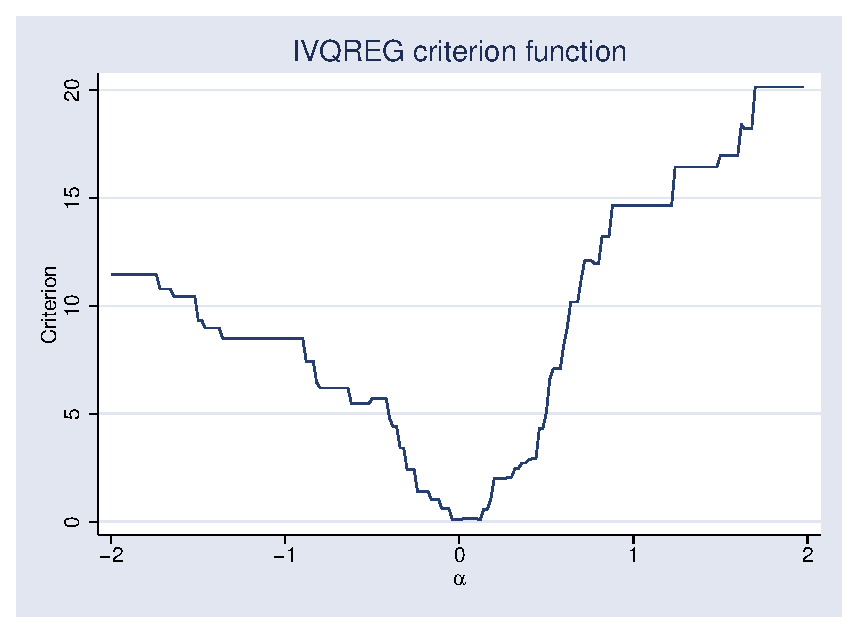
\includegraphics[scale=0.8]{eps/ivqreg_obj}
\caption{IVQREG GMM criterion function}
\end{figure}

For simplicity, the outcome variable only depends on one endogenous variable
$D$, and the true value of $\alpha$ equals to zero. We plot the GMM criterion
function at different values of $\alpha$. While the criterion function is
globally minimized at zero, the plot is flat in certain regions and exhibits
several local minimums. Thus, it is computationally difficult to solve the
optimization problem using the moment condition in Equation \ref{eq:moment3}.



%------------------------------------------------------------------------------
\subsection{Different approaches}	
%------------------------------------------------------------------------------

In literature, there are several estimation approaches to alleviate
the difficulties posed by non-smoothness and non-convexity. We list these
approaches in the chromatic order.

\begin{enumerate}
	\item \cite{Chernozhukov2003}: an MCMC approach.
	\item \cite{Chernozhukov2006}: inverse quantile regression
	\item \cite{Kaplan2017} and \cite{DeCastro2019}: smoothed estimating
	  equation
	\item \cite{Chen2018}: exact GMM via mixed-integer quadratic programming
	\item \cite{Kaido2021}: decentralization
\end{enumerate}

To avoid directly optimizing the original GMM optimization,
\cite{Chernozhukov2003} propose using the Markov Chain Monte Carlo method to
simulate the distribution of the parameter $\thetab$. We can implement this
approach using the {\tt bayesmh}. However, as usually seen in the Bayesian
approach, the estimator's performance may depend on other inputs such as prior
specification.  This method is worth implementation, or at least internally.  It
is interesting to compare the performance of this MCMC method with other
frequentist approaches.

\cite{Chernozhukov2006} propose estimating the IVQR model by conducting a
series of regular quantile regressions, and they name this method as inverse
quantile regression. This method is easy to implement but suffers from the curse
of dimensionality. The inverse quantile regression needs to do a grid search of
dimension $R^{k_d}$. However, this method can efficiently produce estimates at
different quantiles when there are a few endogenous variables. This method should
be implemented as a benchmark because it is already widely used.

\cite{Kaplan2017} and \cite{DeCastro2019} suggest to smooth the indicator
function in Equation \ref{eq:moment3} and then to solve the smoothed GMM
objective function. This method makes the objective function smooth, but the
non-convexity is still there. Thus, to implement this method, we need an
efficient optimization algorithm such as simulated annealing for the nonconvex
problem in Stata. We can use the Mata function {\tt solvenl()} to solve the
estimating equation for the just-identified case.  Compared with the inverse
quantile regression, the main advantage of this method  is that it does not
suffer from the curse of dimensionality. By the way, the over-identified case
can be transformed into a just-identified case by linear projection.

The recent advances of mixed-integer quadratic programming make it possible to
directly solve the nonconvex and nonsmooth optimization problems like Equation
\ref{eq:gmm_original}. \cite{Chen2018} show how to solve the original
GMM objective function in this path. This approach depends on the third-party
package for the mixed-integer quadratic programming algorithm.  Furthermore, 
this method is slow even when the sample size is moderate. 
Given the difficulty of implementing Stata's own mixed-integer quadratic
programming algorithm, we should not implement this method.

Finally, \cite{Kaido2021} propose recasting the original IVQR GMM
optimization problem into an iterative series of regular quantile regression.
The idea is to divide the problem into a simple and easy-to-compute subproblem,
denoting decentralization. The standard errors are obtained via
standard bootstrap. This method is promising because it is easy to implement as
the inverse quantile regression, and it does not suffer from the curse of
dimensionality. Furthermore, this method does not need extra tuning parameters
such as priors in the MCMC approach or the bandwidth choice in the smoothed GMM
approach.  However, this method requires adding the {\tt noconstant} option to
{\tt qreg}. Also, some preliminary simulation results show that this method is
sensitive to the starting values, and it may even be inconsistent when the model
is over-identified.

Considering the different properties of the above approaches, we propose the
following priority order of implementation.

\begin{enumerate}

\item Inverse quantile regression (benchmark)

\item Smoothed EE 

\item Decentralization (postpone due to {\tt noconstant qreg} and
over-identification issues)

\item MCMC approach (postpone)

\end{enumerate}

Section \ref{sec:iqr_method} describes the inverse quantile regression
estimator.  Section \ref{sec:see_method} introduces the smoothed EE estimator.
Finally, section \ref{sec:dec_method} documents the decentralized estimator.



% inverse quantile regression 
%------------------------------------------------------------------------------
\section{Inverse quantile regression} \label{sec:iqr_method}
%------------------------------------------------------------------------------

%------------------------------------------------------------------------------
\subsection{Main results of IQR}	
%------------------------------------------------------------------------------
Rather than directly optimizing the original GMM objective function in Equation
\ref{eq:gmm_original}, \cite{Chernozhukov2006} propose to do a grid search over
$\alphab$, and each step is a regular quantile regression. They label this process
as "inverse quantile regression" (IQR). The intuition is from the moment
condition in the linear IV quantile regression model in Equation
\ref{eq:moment2}. It implies that the $\tau$-th quantile of $Y -
\Db'\alphab$ conditional on $\Xb$ and $\Zb$ is $\Xb'\betab$:
\begin{align}
Q_{Y - \Db'\alphab_0}(\tau |X, Z) = \Xb' \betab_0 +
\widehat{\Phib}(\tau)'\gammab_0, \qquad \text{with } \gammab_0 = 0 \label{eq:IQR}
\end{align}
where $\widehat{\Phib}(\tau)$ is the transformation of $\Zb$ and $\Xb$. In
practice, $\widehat{\Phib}(\tau)$ is the linear projection of $\Db$ on $\Xb$ and
$\Zb$.

Equation \ref{eq:IQR} means that, based on the true value $\alphab_0$, the
conditional quantile regression of $Y-\Db'\alphab_0$ on $\Xb$ and $\Zb$ will
yield the coefficient on $\widehat{\Phib}(\tau)$ to zero.  Given a sequence of
$\alphab$, denoted as $A = \{\alphab_j\}_{j=1}^J$, we just need to run $J$
regular quantile regression of $ y - \Db'\alphab_j$ on $\Xb$ and
$\widehat{\Phib}(\tau)$.  Denote the estimate for $\gammab_j$ as
$\hat{\gammab}(\alphab_j)$.  Then, the estimator $\hat{\alphab}_{IQR}$ for
$\alphab$ is $\alphab_j$ such that $\hat{\gammab}(\alphab_j)$ is the smallest.
Algorithm \ref{algo:iqr} describes the IQR procedure.

\begin{algorithm}[H]
\caption{Inverse quantile regression} \label{algo:iqr}
\begin{enumerate}
    
\item Define a sequence of $\alphab$'s, denoted by $A = \{\alphab_j\}_{j=1}^J$.

\item Define the quantile level $\tau$.

\item For each variable in $\Db$, compute its linear projection on the space
spanned by $\Xb$ and $\Zb$. Denote the predicted $\Db$ as $\widehat{\Phib}$.

\item For $j$ from $1$ to $J$, make the following loop.

\begin{enumerate}
	\item Run regular $\tau$-th quantile regression of $Y - \Db'\alphab_j$ on
	$\Xb$ and $\widehat{\Phib}$. Denote the estimate for $\betab$ and
	$\gammab$ as $\hat{\betab}(\alphab_j)$ and $\hat{\gammab}(\alphab_j)$,
	respectively.  Also denote the $\hat{\Omegab}(\alphab_j)$ as the estimated
	variance matrix for $\sqrt{N}(\hat{\gammab}(\alphab_j) -
	\gammab(\alphab_j))$.

	\item Compute the norm of $\hat{\gammab}(\alphab_j)$ as $W(\alphab_j) =
	N\hat{\gammab}(\alphab_j)' \hat{\Omegab}(\alphab_j)^{-1}
	\hat{\gammab}(\alphab_j)$
\end{enumerate}

\item The IQR estimate for $\alphab$ is $\hat{\alphab}_{IQR}$ such that
$W(\hat{\alphab}_{IQR})$ is the smallest among $\{W(\alphab_j)\}_{j=1}^J$.
Formally,
\begin{align*}
	\hat{\alphab}_{IQR} = \argmin_{\alphab \in A} W(\alphab)
\end{align*}

\item Given $\hat{\alphab}_{IQR}$, the estimate for $\betab$ is
$\hat{\betab}(\hat{\alphab}_{IQR})$.

\end{enumerate}
\end{algorithm}

\vskip 1cm
To obtain the standard error of the IQR estimator, we have the following
theorem.

\begin{theorem}
\label{thm:iqr_var}
(Theorem 3 in \cite{Chernozhukov2006})
Given some regularity assumptions, for $\epsilon_i(\tau) = Y_i -
\Db_i'\alphab(\tau) - \Xb_i'\betab(\tau)$ and 
$l_i(\tau, \thetab(\tau)) = (\tau - \I (\epsilon_i(\tau) <0))$, 
where $\thetab = (\alphab(\tau), \betab(\tau))$;

\begin{align}
\sqrt{n}(\hat{\thetab}(\cdot) - \thetab(\cdot))
=
- \Jb(\cdot)^{-1} \frac{1}{\sqrt{n}} \sum_{i=1}^n l_i(\cdot,
  \thetab(\cdot))\Psib_i(\cdot) + o_p(1) \implies \bb(\cdot)
\end{align}
where $\bb(\cdot)$ is a mean zero Gaussian process with covariance function
\begin{align*}
\E \bb(\tau) \bb(\tau')' &= \Jb(\tau)^{-1} \Sb(\tau, \tau') [\Jb(\tau')^{-1}]'
\\ \intertext{and}
\Psib_i(\tau) &= (\Phib_i(\tau)', \Xb_i')' \\
\Jb(\tau) &= \E\left[
f_{\epsilon(\tau)}(0|\Xb, \Db, \Zb)\Psib(\tau) [\Db', \Xb']
\right] \\
\Sb(\tau, \tau') &= (\min(\tau, \tau') - \tau \tau') \E \Psib(\tau) \Psib(\tau)'
\end{align*}
where $f_{\epsilon(\tau)}(0| \Xb, \Db, \Zb)$ is the conditional density of
$\epsilon(\tau)$ evaluated at zero.
\end{theorem}

For a discussion on the intuition behind Theorem \ref{thm:iqr_var}, see Section
\ref{sec:discuss_iqrvar}

\begin{remark} \label{iqr:dist} (Remark 3 in \cite{Chernozhukov2006})
A basic implication of Theorem \ref{thm:iqr_var} is that for a given probability
index $\tau$
\begin{align}
	\sqrt{n}(\widehat{\thetab}(\tau) - \thetab(\tau))
	\to N(0, \Jb(\tau)^{-1} \Sb(\tau, \tau) [\Jb(\tau)^{-1}]')
	\label{eq:iqr_var}
\end{align}
Also, for any finite collection of quantile indices ${\tau_j, j \in T}$
\begin{align}
	\{\sqrt{n}(\widehat{\thetab}(\tau) - \thetab(\tau)) \}_{j\in T}
	\to N(0, \{ \Jb(\tau_k)^{-1} \Sb(\tau_k, \tau_l)
	[\Jb(\tau_l)^{-1}]'\}_{k, l \in T})
	\label{eq:iqr_var_tau}
\end{align}
\end{remark}

\begin{remark} \label{iqr:vce} (Remark 4 in \cite{Chernozhukov2006})
The components in the variance matrix in (\ref{eq:iqr_var}) and
(\ref{eq:iqr_var_tau}) can be obtained by its sample counterparts:
\begin{align}
	\widehat{\Sb}(\tau, \tau') = (\min(\tau, \tau') - \tau \tau')
		\frac{1}{n}\sum_{i=1}^n\widehat{\Psib}_i\widehat{\Psib}_i'
\end{align}

The estimator for $\Jb(\tau)$ takes the form
\begin{align}
	\frac{1}{n h_n}\sum_{i}^n K\left(\frac{- \epsilon_i(\tau)}{h_n}\right)
	\widehat{\Psib}_i[\Db_i', \Xb_i']
\end{align}
where $K(\cdot)$ is a Kernel function and $h_n$ is the bandwidth.
\end{remark}
In practice, we can use Kernel as in Stata command {\tt kdensity}. 
For example, the Gaussian Kernel is
$$
K(z) = \frac{1}{\sqrt{2\pi}}e^{-\frac{z^2}{2}}
$$


For the bandwidth, we can use either the Silverman's rule of thumb bandwidth or
the bandwidth used \citeauthor{Koenker2005} (\citeyear{Koenker2005}, Page 81).

The Silverman's rule of thumb bandwidth is 
\begin{align}
  h_{s} = 0.9 
  \min\left(\widehat{\sigma(\epsilon)}, \frac{M}{1.349}\right) 
  n^{-\frac{1}{5}}
\end{align}
where $\widehat{\sigma(\epsilon)}$ is the standard deviation of $\epsilon$ and
$M$ is the interquartile range of $\epsilon$.

The Koenker bandwidth is 
\begin{align}
  h_{k} = 
  \min\left(\widehat{\sigma(\epsilon)}, \frac{M}{1.349}\right) 
  (\Phi^{-1}(\tau + h_1) - \Phi^{-1}(\tau - h_1))
\end{align}
where $h_1$ can be one of the bandwidth in \cite{Hall1988} and
\cite{Bofinger1975}. In particular, 
\begin{align}
	h_{hs} &= n^{-1/3}\Phi^{-1}\left(1 - \frac{\alpha}{2}\right)^{2/3}
	\left[
	\frac{3}{2}\times
	\frac{\phi\left\{\Phi^{-1}(\tau)\right\}^2}
	{2 \Phi^{-1}(\tau)^2 + 1}
\right]^{1/3}
\\
	h_{b} &= n^{-1/5}
	\left[
	\frac{9}{2}\times
	\frac{\phi\left\{\Phi^{-1}(\tau)\right\}^4}
	{\left\{2 \Phi^{-1}(\tau)^2 + 1\right\}^2}
\right]^{1/5}
\end{align}


%------------------------------------------------------------------------------
\subsection{Robust inference approach} \label{sec:iqr_robust}
%------------------------------------------------------------------------------
In the presence of weak instruments the inference is
unreliable. \cite{Chernozhukov2008} proposed an inference approach robust to the
weak instruments. In addition, this approach allows evaluating the quality of
grid specification so that the grid covers the true value of $\alphab$ with a
predefined probability level. 

\begin{prop} \label{prop:robust} (Proposition 1 in \cite{Chernozhukov2008})
When $\alphab =  \alphab(\tau)$,
\begin{align*}
  W_n[\alphab(\tau)] \rightarrow_d \chi^2(dim(\gammab))
\end{align*}
and for the confidence region $CR_p[\alphab(\tau)] = \{\alphab \in A:
W_n(\alphab) < c_p\}$, where $P(\chi^2(dim(\gammab)) < c_p) = p$,
\begin{align}
  P\{\alphab(\tau) \in CR_p[\alphab(\tau)]\} = P\{ W_n[\alphab(\tau)] < c_p\} =
  p
\end{align}
\end{prop}

Intuitively, $W_n(\alphab(\tau))$ is the Wald statistic for testing whether the
coefficients for the instruments are zero ($\hat{\gammab} = 0$). When $\alphab$
equals the true value $\alphab(\tau)$, $W(\cdot)$ is $\chi^2$
distributed with the degree of freedom of dimension of $\gammab$. Thus a valid
confidence interval for $\alphab$ can be constructed by the inversion of the
Wald statistic. That is 
$$
CR_p[\alphab(\tau)] = \{\alphab \in A: W_n(\alphab) < c_p\}
\text{ cover the true value of $\alphab$ with probability approaching
$p$}
$$

The confidence region is a byproduct of the inverse quantile regression.
Algorithm \ref{algo:iqr_robust} is an extension of algorithm \ref{algo:iqr} so
that the robust confidence region is computed. Following
\cite{Chernozhukov2008}, the robust confidence interval $CR_p$ is also called 
dual confidence interval, abbreviated as dual CI.

\begin{algorithm}[H]
\caption{Inverse quantile regression with robust inference}
\label{algo:iqr_robust}

\begin{enumerate}
    % import the iqr algorithm
  
\item Define a sequence of $\alphab$'s, denoted by $A = \{\alphab_j\}_{j=1}^J$.

\item Define the quantile level $\tau$.

\item For each variable in $\Db$, compute its linear projection on the space
spanned by $\Xb$ and $\Zb$. Denote the predicted $\Db$ as $\widehat{\Phib}$.

\item For $j$ from $1$ to $J$, make the following loop.

\begin{enumerate}
	\item Run regular $\tau$-th quantile regression of $Y - \Db'\alphab_j$ on
	$\Xb$ and $\widehat{\Phib}$. Denote the estimate for $\betab$ and
	$\gammab$ as $\hat{\betab}(\alphab_j)$ and $\hat{\gammab}(\alphab_j)$,
	respectively.  Also denote the $\hat{\Omegab}(\alphab_j)$ as the estimated
	variance matrix for $\sqrt{N}(\hat{\gammab}(\alphab_j) -
	\gammab(\alphab_j))$.

	\item Compute the norm of $\hat{\gammab}(\alphab_j)$ as $W(\alphab_j) =
	N\hat{\gammab}(\alphab_j)' \hat{\Omegab}(\alphab_j)^{-1}
	\hat{\gammab}(\alphab_j)$
\end{enumerate}

\item The IQR estimate for $\alphab$ is $\hat{\alphab}_{IQR}$ such that
$W(\hat{\alphab}_{IQR})$ is the smallest among $\{W(\alphab_j)\}_{j=1}^J$.
Formally,
\begin{align*}
	\hat{\alphab}_{IQR} = \argmin_{\alphab \in A} W(\alphab)
\end{align*}

\item Given $\hat{\alphab}_{IQR}$, the estimate for $\betab$ is
$\hat{\betab}(\hat{\alphab}_{IQR})$.


  \item The dual confidence region for $\alphab(\tau)$, $CR_p$, can be computed
    as $CR_p[\alphab(\tau)]  = \{ \alphab_j : W_n(\alphab_j) < c_p \}$, where
    $P(\chi^2(dim(\gammab)) < c_p) = p$. By default, $p = 0.95$.  The upper and
    lower bound of $CR_p(\alphab(\tau)$ may be used as endpoints of confidence
    interval for $\alphab(\tau)$

  \item If $CR_p$ is empty, $\Ab$ is not a valid grid specification because the
    true value of $\alphab(\tau)$ is not covered by $\Ab$ with a big probability.

\end{enumerate}

\end{algorithm}

%------------------------------------------------------------------------------
\subsection{Initial grid}
%------------------------------------------------------------------------------
The initial grid points are computed using the two-stage-quantile regression,
extending the two-stage-median regression in \cite{Amemiya1982}.
The quality of the initial grid can be evaluated using the dual CI. The
implementation requires that the initial grid interval be wider than the
dual CI. Otherwise, {\tt ivqregress iqr} will error out.

A simulation is run to evaluate the effectiveness of the dual CI. In particular,
in a repeated sampling setting, we compute the coverage rate of the dual CI.  In
each repetition, we compute the coverage indicator, which is either 1 if the
true value is within the dual CI or 0 otherwise. The coverage is the average of
the indicator variable over $1000$ repetitions. The sample size is set to
$1000$.  Given the default 95\% level, the coverage rate of the dual CI should
be close to $0.95$. Figure \ref{fig:dualci} plots the coverage rate of dual CI
at different quantile estimates. As expected, the dual CI can cover the
true value with a probability close to $95\%$.

\begin{figure}[H]
\caption{dual 95\% CI coverage rate}
\label{fig:dualci}
\centering
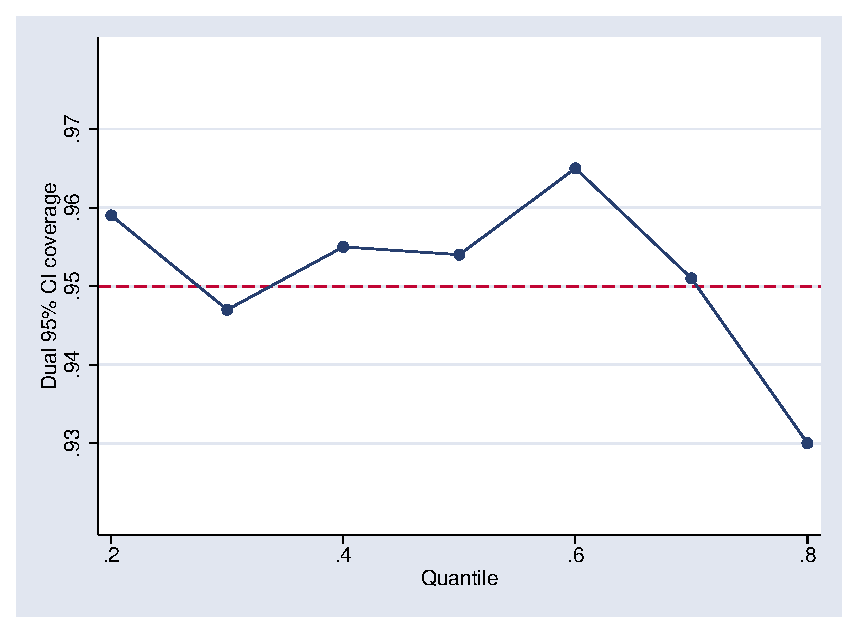
\includegraphics[scale=0.8]{eps/dualci}
\end{figure}

The two-stage-quantile regression is computed in the following steps.

\begin{enumerate}
  \item Compute $\hat{\Phib}(\tau)$, which is the linear projection of $\Db$ on
  $\Xb$ and $\Zb$.
  \item Run a quantile regression of $Y$ on $\Xb$ and $\hat{\Phib}(\tau)$.
  Denote $\tilde{\alphab}$ as the point estimates for the coefficient on
  $\hat{\Phib}(\tau)$ and $\tilde{s}$ as its standard errors.  $\tilde{s}$ is
  computed by assuming the error term is normally distributed.
  \item Compute the lower and upper bound of the grid. The lower bound is
    $lb = \tilde{\alphab} - 4\tilde{s}$, and the upper bound is 
    $ub = \tilde{\alphab} + 4\tilde{s}$.
  \item By default, the grid points are 30 equally spaced points between $lb$
  and $ub$. We can also specify the number of grid points in option {\tt
  ngrid()}.
\end{enumerate}

We show one example to illustrate the connection between the dual CI
and the grid.  To fix the idea, we fit an IVQR model using the simulated data.
First, we fit the inverse quantile regression of $y$ on the endogenous $d1$ and
exogenous $x1$ and $x2$, and use $z1$ and $z2$ as instruments.

\begin{stlog}
. ivqregress iqr y x1 x2 (d1 = z1 z2),  quantile(40) noadaptive
{\smallskip}
Initial grid
    quantile = 0.40: .........10.........20.........30
{\smallskip}
IV .4 quantile regression                              Number of obs =   1,000
Estimator: Inverse quantile regression                 Wald chi2(3)  = 3534.04
                                                       Prob > chi2   =  0.0000
{\smallskip}
\HLI{13}{\TOPT}\HLI{64}
             {\VBAR}               Robust
           y {\VBAR} Coefficient  std. err.      z    P>|z|     [95\% conf. interval]
\HLI{13}{\PLUS}\HLI{64}
          d1 {\VBAR}    .459274   .0502662     9.14   0.000      .360754    .5577939
          x1 {\VBAR}   1.393901   .0334069    41.72   0.000     1.328425    1.459377
          x2 {\VBAR}   1.427885   .0321419    44.42   0.000     1.364888    1.490882
       _cons {\VBAR}  -.3458003   .0411389    -8.41   0.000     -.426431   -.2651695
\HLI{13}{\BOTT}\HLI{64}
Endogenous: d1
 Exogenous: x1 x2 z1 z2
{\smallskip}

\end{stlog}

By default, the initial grid is computed by the two-stage-quantile regression.
We now plot the Wald statistic for each point in the grid. 

\begin{stlog}
. estat waldplot

\end{stlog}

\begin{figure}[H]
\caption{Wald statistic plot}
\label{fig:dualci}
\centering
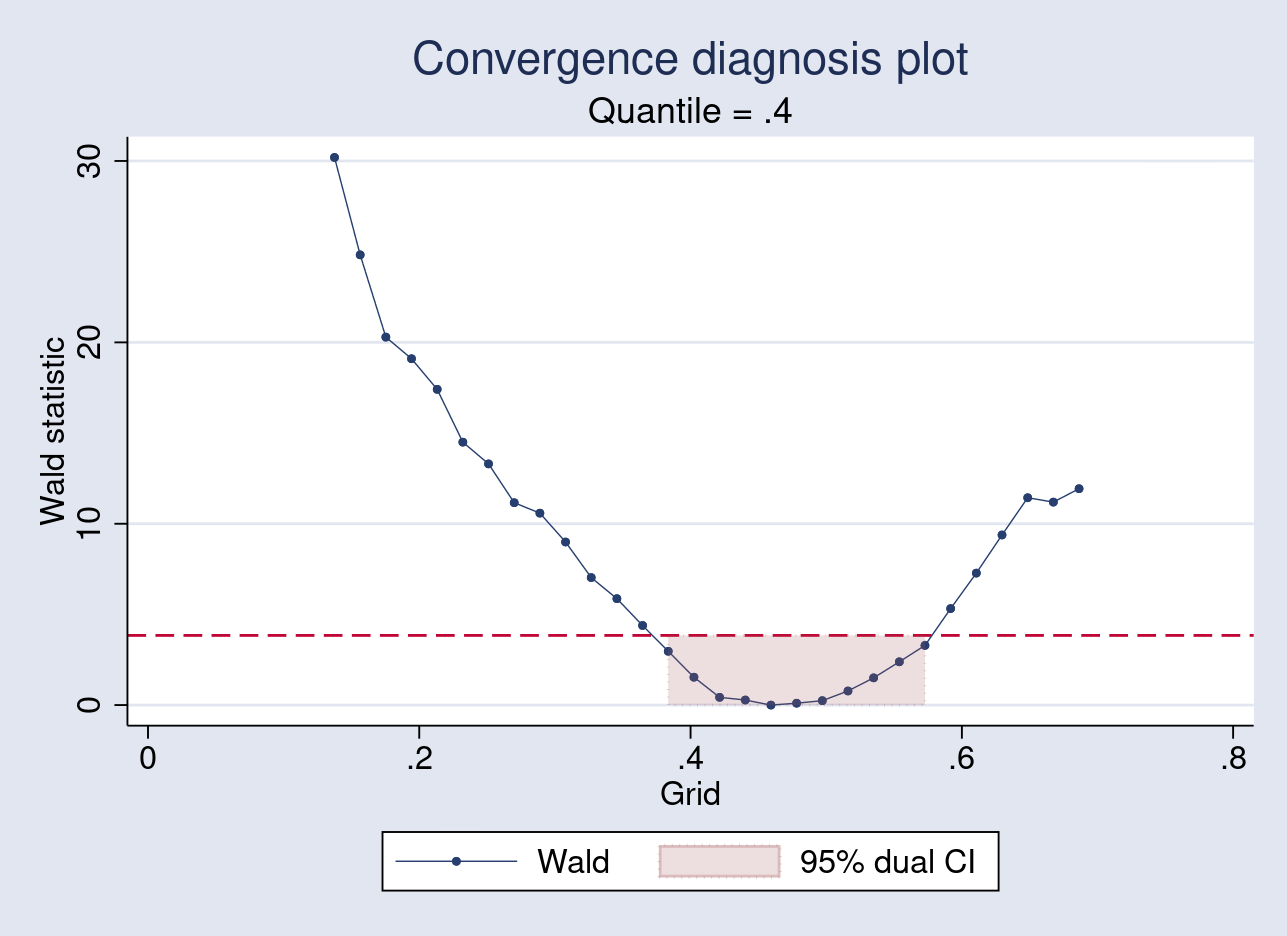
\includegraphics[scale=0.3]{eps/waldplot}
\end{figure}

In the above graph, the Wald statistics are plotted for each point in the grid.
The critical value of the Wald statistic is shown as a red horizontal dash line.
The dual CI is the grid points such that the corresponding Wald statistic is
smaller than the critical value, shown in the red shaded area. 

From the above graph, we can visually inspect two features regarding the
estimation. First, we see that the point estimate results in the minimum of the
Wald statistic. Second, we see that the point estimate is within the $95\%$ dual
CI and the initial grid interval is wider than the dual CI. Thus, we are $95\%$
or more confident that the initial grid interval contains the true value of the
parameter.

To see the numerical values of the dual CI, we use {\tt estat dualci}.

\begin{stlog}
. estat dualci
{\smallskip}
Dual confidence interval                                 Number of obs = 1,000
\HLI{13}{\TOPT}\HLI{64}
             {\VBAR}               Robust                               Dual
           y {\VBAR} Coefficient  std. err.      z    P>|z|     [95\% conf. interval]
\HLI{13}{\PLUS}\HLI{64}
          d1 {\VBAR}    .459274   .0502662     9.14   0.000     .3835663    .5728356
\HLI{13}{\BOTT}\HLI{64}

\end{stlog}

%------------------------------------------------------------------------------
\subsection{Adaptive grid search}
%------------------------------------------------------------------------------
Sometimes, a point estimate is found in a flat region, which implies some
degree of weak identification of the parameter. The weak identification can be
caused by the weak identified model or the coarse grid points. The
adaptive grid search can help alleviate the weak identification issue caused by
the coarse grid points. However, the adaptive grid search can not help if the
model is intrinsically weakly identified.

The adaptive grid search is conducted in the following steps.

\begin{enumerate}
  \item Based on the initial grid points, compute the inverse quantile
    regression and the dual CI. 
  \item Construct a new grid using the dual CI, that is, construct several
    equally spaced points between the lower and upper bound in the dual CI.
  \item Compute the inverse quantile regression using the grid in 
    step 2.
\end{enumerate}

Here is one example. First, we fit a IVQR model using the original grid and
plot the Wald statistics.

\begin{stlog}
. use assets2, clear
(Excerpt from Chernozhukov and Hanson (2004) Rev. of Economics and Statistics)
{\smallskip}
. 
. ivqregress iqr assets (i.p401k = i.e401k) income age familysize ///
>         i.married i.ira i.pension i.ownhome educ, quantile(50) noadaptive
{\smallskip}
Initial grid
    quantile = 0.50: .........10.........20.........30
{\smallskip}
IV median regression                                   Number of obs =   9,913
Estimator: Inverse quantile regression                 Wald chi2(9)  = 1312.24
                                                       Prob > chi2   =  0.0000
{\smallskip}
\HLI{13}{\TOPT}\HLI{64}
             {\VBAR}               Robust
      assets {\VBAR} Coefficient  std. err.      z    P>|z|     [95\% conf. interval]
\HLI{13}{\PLUS}\HLI{64}
     1.p401k {\VBAR}   5073.007   551.8459     9.19   0.000     3991.409    6154.605
      income {\VBAR}    .159635   .0124353    12.84   0.000     .1352622    .1840077
         age {\VBAR}   100.7959   8.584905    11.74   0.000     83.96984     117.622
  familysize {\VBAR}  -203.4073   54.42447    -3.74   0.000    -310.0773   -96.73727
             {\VBAR}
     married {\VBAR}
    Married  {\VBAR}  -1348.987   227.0043    -5.94   0.000    -1793.907   -904.0668
             {\VBAR}
         ira {\VBAR}
        Yes  {\VBAR}   22630.45   1016.463    22.26   0.000     20638.21    24622.68
             {\VBAR}
     pension {\VBAR}
Receives ..  {\VBAR}  -708.9357   210.4489    -3.37   0.001    -1121.408   -296.4633
             {\VBAR}
     ownhome {\VBAR}
        Yes  {\VBAR}  -39.62138   154.8029    -0.26   0.798    -343.0294    263.7867
        educ {\VBAR}  -98.81898   32.18152    -3.07   0.002    -161.8936   -35.74435
       _cons {\VBAR}  -5026.207    570.501    -8.81   0.000    -6144.368   -3908.045
\HLI{13}{\BOTT}\HLI{64}
Endogenous: 0b.p401k 1.p401k
 Exogenous: income age familysize 0b.married 1.married 0b.ira 1.ira
            0b.pension 1.pension 0b.ownhome 1.ownhome educ 0b.e401k 1.e401k
{\smallskip}
. 
. estat waldplot, name(a)

\end{stlog}

\begin{figure}[H]
\caption{Wald statistic plot}
\label{fig:dualci}
\centering
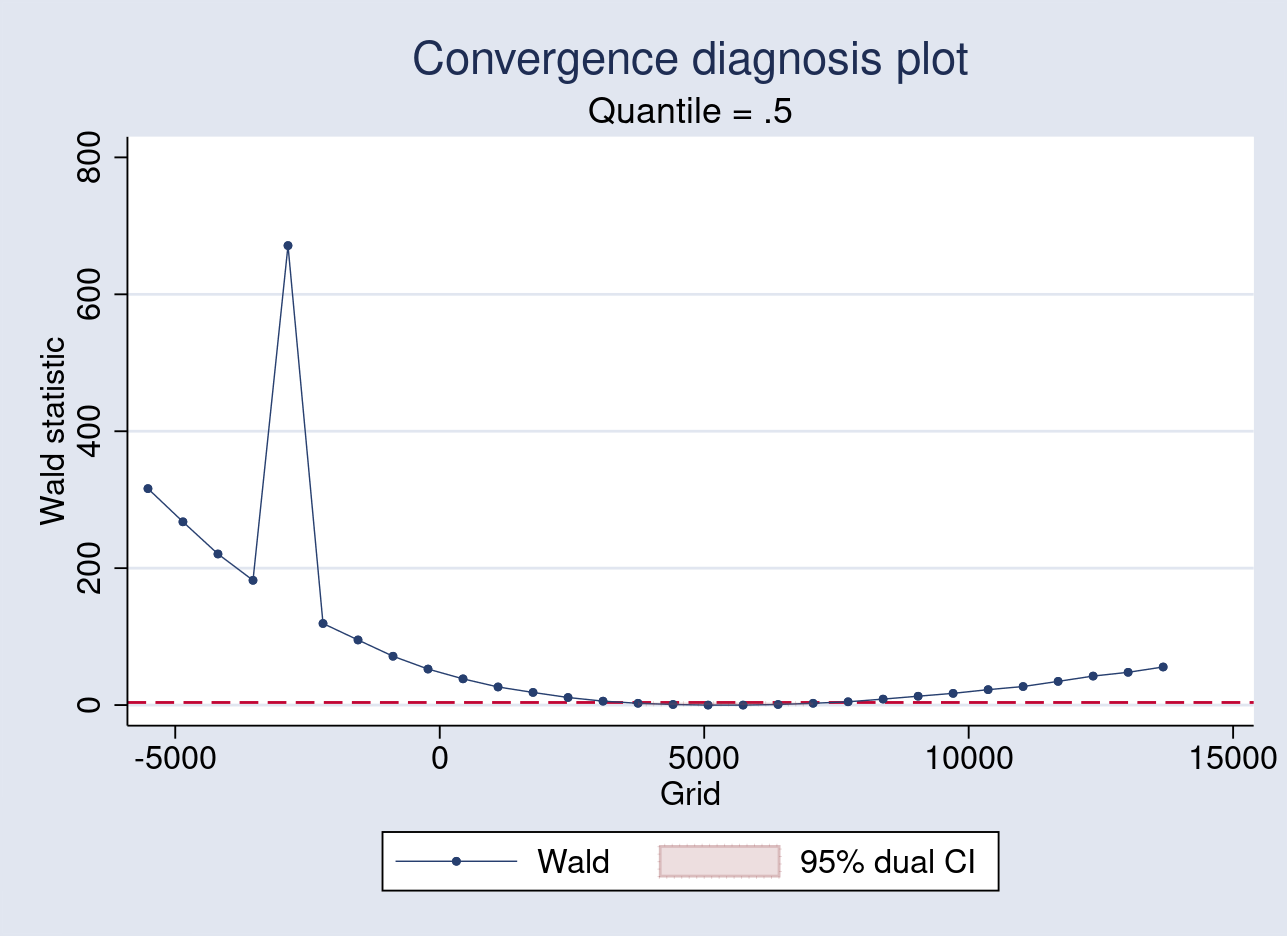
\includegraphics[scale=0.3]{eps/waldplot_asset}
\end{figure}

The Wald plot shows that the minimum is found in a flat region. Now, we refit
the IVQR model but using the adaptive grid search.

\begin{stlog}
. use assets2, clear
(Excerpt from Chernozhukov and Hanson (2004) Rev. of Economics and Statistics)
{\smallskip}
. 
. ivqregress iqr assets (i.p401k = i.e401k) income age familysize ///
>         i.married i.ira i.pension i.ownhome educ, quantile(50) 
{\smallskip}
Initial grid
    quantile = 0.50: .........10.........20.........30
{\smallskip}
Adaptive grid
    quantile = 0.50: .........10.........20.........30
{\smallskip}
IV median regression                                   Number of obs =   9,913
Estimator: Inverse quantile regression                 Wald chi2(9)  = 1289.75
                                                       Prob > chi2   =  0.0000
{\smallskip}
\HLI{13}{\TOPT}\HLI{64}
             {\VBAR}               Robust
      assets {\VBAR} Coefficient  std. err.      z    P>|z|     [95\% conf. interval]
\HLI{13}{\PLUS}\HLI{64}
     1.p401k {\VBAR}   5313.397   573.2818     9.27   0.000     4189.786    6437.009
      income {\VBAR}   .1577512   .0124889    12.63   0.000     .1332735    .1822289
         age {\VBAR}   99.96526   8.561923    11.68   0.000      83.1842    116.7463
  familysize {\VBAR}  -197.8251   54.36773    -3.64   0.000    -304.3838   -91.26627
             {\VBAR}
     married {\VBAR}
    Married  {\VBAR}  -1359.124   227.3366    -5.98   0.000    -1804.696   -913.5528
             {\VBAR}
         ira {\VBAR}
        Yes  {\VBAR}   22629.61   1022.706    22.13   0.000     20625.15    24634.08
             {\VBAR}
     pension {\VBAR}
Receives ..  {\VBAR}  -693.8347   210.6176    -3.29   0.001    -1106.638   -281.0317
             {\VBAR}
     ownhome {\VBAR}
        Yes  {\VBAR}  -30.29657   154.7265    -0.20   0.845     -333.555    272.9618
        educ {\VBAR}  -96.43983   32.09465    -3.00   0.003    -159.3442   -33.53547
       _cons {\VBAR}  -4998.673   570.1315    -8.77   0.000     -6116.11   -3881.236
\HLI{13}{\BOTT}\HLI{64}
Endogenous: 0b.p401k 1.p401k
 Exogenous: income age familysize 0b.married 1.married 0b.ira 1.ira
            0b.pension 1.pension 0b.ownhome 1.ownhome educ 0b.e401k 1.e401k
{\smallskip}
. 
. estat waldplot, name(b)

\end{stlog}

\begin{figure}[H]
\caption{Wald statistic plot}
\label{fig:dualci}
\centering
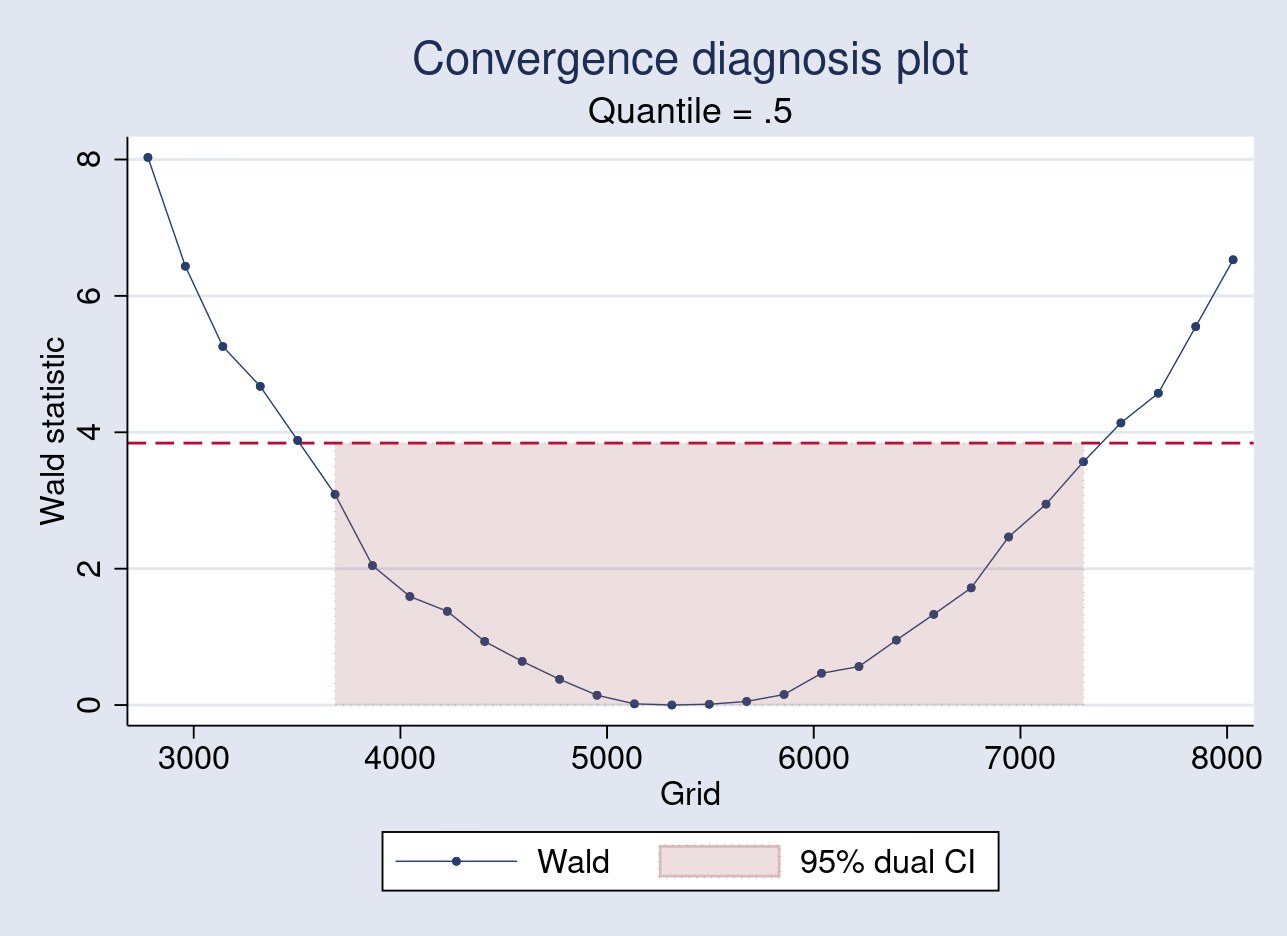
\includegraphics[scale=0.3]{eps/waldplot_asset2}
\end{figure}

Clearly, the adaptive grid search helps to identify the point estimate in a more
convex region.  By default, {\tt ivqregress iqr} is doing a robust and
adaptive grid search.



% smoothed estimating equation 
%------------------------------------------------------------------------------
\section{Smoothed estimating equation estimator}\label{sec:see_method}
%------------------------------------------------------------------------------
The basic idea of smoothd estimating equation (SEE) estimator for the IVQR
model is to replace the indicator function in the moment condition with a smooth
function. To be precise, we replace the moment condition in Equation
(\ref{eq:moment2}) with
\begin{align}
\frac{1}{n}\sum_{i=1}^n \left[ \tau - \Is (Y_i  - \Db_i'\alphab - \Xb_i'\betab
\leq 0) \right] \Psib_i(\Xb, \Zb) = 0 \label{eq:moment_sgmm}
\end{align}
where $\Is()$ is defined as
\begin{align}
\Is(v) & =
\begin{cases}
  1 & \text{if $v \leq -1$} \\
  0 & \text{if $v \geq 1$}\\
  \frac{1-v}{2} &\text{if $-1 < v < 1$}
\end{cases}
\label{eq:Is}
\end{align}
Mathematically, $\Is() = \max\{0, \min\{1, \frac{1-v}{2}\}\}$.

Figure \ref{fig:sgmm} plot the $\Is(v/h)$ with different bandwidth $h$. We see
that smaller bandwidth approximate the indicator function better.

\begin{figure}[H]
\caption{Smoothed indicator function}
\label{fig:sgmm}
\centering
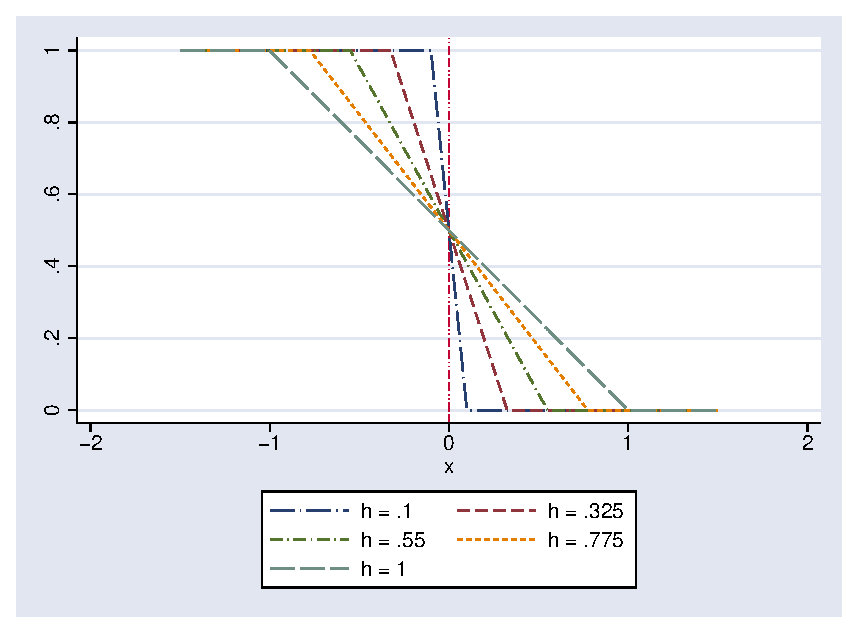
\includegraphics[scale=0.8]{eps/i_sgmm}
\end{figure}

Here are some remarks on the smoothed EE estimator.

\begin{itemize}
  \item In practice, $\Psib(\Xb, \Zb) = (\Xb', \Phib(\Xb, \Zb)')'$, and
    $\Phib(\Xb, \Zb)$ can be computed as the linear projection of $\Db$'s on the
    space spanned by $\Xb$ and $\Zb$. So, the over-identified model can 
    be transformed to a just-identified model. 

  \item Given a bandwidth $h$, the solution to Equation (\ref{eq:moment_sgmm})
    can be found via mata function {\ty solvenl()}. 

  \item The SEE estimator does not suffer from the curse of dimensionality as
    seen in the inverse quantile regression estimator.
\end{itemize}

%------------------------------------------------------------------------------
\subsection{Optimal bandwidth}
%------------------------------------------------------------------------------
The optimal bandwidth minimize the asymptotic MSE of the smoothed estimating
equations. For details, see Proposition 2 in \cite{Kaplan2017}.

The optimal bandwidth $\hsee$ is defined as
\begin{align}
  \hsee & = 
\left(
\frac{(r!)^2 \left[ 1- \int_{-1}^{1}G^2(u)du \right] f_U(0)}
{2r \left[\int_{-1}^1 G'(v)v^rdv \right]^2 
\left[f_U^{(r-1)}(0) \right]^2} \frac{p}{n}\right)^{\frac{1}{2r - 1}}
\end{align} 

where 
\begin{itemize}
  \item $G(u) = \Is(-u)$ 
  \item $r$ means $G(u)$ is a bounded $r$th order kernel such that $\int_{-1}^1
    v^k G'(v)dv = 0$ for $k = 1, 2, \ldots, r-1$ and $\int_{-1}^1 |v^r G'(v)dv|
    < \infty$. In the case of $\Is()$, $r = 2$.
  \item $p$ is the sum of the dimension of $\betab$ and $\alphab$.
  \item $U = Y - \Db'\alphab - \Xb'\betab$ and $f_U(0)$ is the PDF of
    $U$ at the point $0$.
  \item $f^{(1)}_U(0)$ is the derivatives of the PDF of $U$ evaluated at the
    point $0$.
\end{itemize}

Given the definition of $\Is()$ in Equation (\ref{eq:Is}), we can further
simplify the expression of $\hsee$. In particular,
\begin{align*}
1- \int_{-1}^{1}G^2(u)du 
&= 1 - \int_{-1}^1 \frac{(1 + v)^2}{4}dv = 1 - \frac{(1+v)^3}{12}|_{-1}^{1}
= \frac{1}{3} \\
\left[ \int_{-1}^1 G'(v)v^rdv  \right]^2
&=\left[ \int_{-1}^1 \frac{v^2}{2}dv \right]^2  
= \left[ \frac{v^3}{6}|_{-1}^1 \right]^2
= \left[ \frac{1}{6} - \frac{-1}{6} \right]^2 = \frac{1}{9}
\end{align*}
Plug in these two values into $\hsee$, we have
\begin{align}
  \hsee & = 
\left(
\frac{(2!)^2 \frac{1}{3}f_U(0)}
{2*2 \frac{1}{9} 
\left[f_U^{(2-1)}(0) \right]^2} \frac{p}{n}\right)^{\frac{1}{2*2 - 1}} \nonumber
\\
&= 
\left(
\frac{3f_U(0)}{\left[f_U^{'}(0) \right]^2} \frac{p}{n}\right)^{\frac{1}{3}} 
\nonumber \\
&= \left( \frac{3p}{n} \right)^{\frac{1}{3}} 
\left(\frac{f_U(0)}{\left[f'_U(0)\right]^2} \right)^{\frac{1}{3}}
\label{eq:bwopt}
\end{align}
Notice that the term $\left( \frac{3p}{n} \right)^{\frac{1}{3}}$ can be used as
an initial value of the bandwidth. We can nonparametrically or parametrically
estimate $f_U(0)$ and $f_U'(0)$. 

%------------------------------------------------------------------------------
\subsection{Nonparametrically estimated optimal bandwidth}
%------------------------------------------------------------------------------
The optimal bandwidth in Equation (\ref{eq:bwopt}) requires the evaluation of
$f_U(0)$ and $f_U'(0)$. Both terms can be estimated using a Kernel-based method.

For $f_U(0)$, given an initial estimate of residuals $\hat{u_i} = Y_i 
-\Db_i'\hat{\alphab}(\tau) -\Xb_i'\hat{\betab}(\tau)$, the kernel density
estimator is 
\begin{align}
  \frac{1}{ns}\sum_{i=1}^n K(\frac{-\hat{u}_i}{s})
\end{align}
where $s$ is the kernel bandwidth and $K()$ is the Gaussian Kernel.

Following the point-wise optimal bandwidth approach in \cite{DasGupta2008} and the
Gaussian reference approach in \cite{Silverman1998}, the optimal $s^*$ is

\begin{align}
  s^* = \left(\frac{1}{2n\sqrt{\pi}}\right)^{1/5}
  \sigma \left\{\phi(\Phi^{-1}(\tau))
  [\left( \Phi^{-1}(\tau) \right)^2 - 1 ]^2 \right\}^{-1/5}
\end{align}
where $\phi()$ is standard Normal density function and $\Phi()$ is standard
Normal CDF. $\sigma$ can be replaced by the sample deviation of the $\hat{u}$
or the standard normal interquartile range, whichever is smaller. 

For the density derivative $f'_U(0)$, the kernel estimator is 
\begin{align}
  \frac{1}{nb^2} \sum_{i=1}^n K'(-\hat{u}_i/b)
\end{align}
, where $K'()$ is the derivative of the Gaussian Kernel.

Following \cite{Wand1995}, the optimal bandwidth $b^*$ can be estimated as 
\begin{align}
b^* =  n^{-1/7}\sigma
\left(
\frac{3/(4\sqrt{\pi})}{
\phi(\Phi^{-1}(\tau)) 
\left[
\Phi^{-1}(\tau)
\right]^2
\left[3 - [\Phi^{-1}(\tau)]^2 \right]^2
}
\right)^{1/7}
\end{align}


%------------------------------------------------------------------------------
\subsection{Parametrically estimated optimal bandwidth}
%------------------------------------------------------------------------------
The optimial bandwidth in Equation (\ref{eq:bwopt}) can also be estimated
parametrically. Assuming the residuals $u$ follows a specific distribution,
the terms $f_U(0)$ and $f'_U(0)$ can be computed.

Suppose $u$ follows a Gaussian distribution, the optimal bandwidth can be
simplified as
\begin{align}
  \hsee =
  n^{-1/3}\sigma
  \left(
  	\frac{3 k_d}
	{
	  \{\Phi^{-1}(\tau)\}^2 \phi(\Phi^{-1}(\tau))
      }
      \right)^{1/3}
\end{align}


%------------------------------------------------------------------------------
\subsection{Detection of ``bad'' bandwidth}
%------------------------------------------------------------------------------
Given any bandwidth $h$, the SEE estimator may or may not converge. A ``bad''
bandwidth means that the SEE estimator does not converge or the SEE estimator
converges, but the point estimates are out of 95\% dual confidence interval. In
the first scenario, the non-convergence issue can be detected easily.  We can
employ the ``robust'' inference approach in \cite{Chernozhukov2008} in the
second scenario. For a detailed discussion, see Section \ref{sec:iqr_robust}.

In particular, we run an auxiliary quantile regression of $Y -
\Db'\hat{\alpha}_{SEE}$ on $\Xb$ and $\Phib(\Xb, \Zb)$, where
$\hat{\alpha}_{SEE}$ is SEE estimates for $\alphab$. Denote the $W_{h}$ as the
Wald statistic for the coefficient on $\Phib(\Xb, \Zb)$. If $W_h$ is greater
than the critical value $c_p$, the point estimates for the endogenous
coefficients are out of the $95\%$ confidence interval.



%------------------------------------------------------------------------------
\subsection{Variance-covariance estimation}
%------------------------------------------------------------------------------
The SEE estimator has the same (first-order) asymptotic distribution and
covariance structure as the inverse quantile regression estimator.  See the
second equation in Theorem 5 in \cite{DeCastro2019} for the derivation.  It
turns out that the SEE estimator in \cite{Kaplan2017} is a special case of the
\cite{DeCastro2019} when assuming the linear IVQR model.  The formulas for the
asymptotic variance estimator are the same as in Remarks \ref{iqr:dist} and
\ref{iqr:vce}. 

Bootstrap can also be used to compute the standard errors.


% general inference
%------------------------------------------------------------------------------
\section{General inference} \label{sec:infer}
%------------------------------------------------------------------------------
We outline the inference procedures in \cite{Chernozhukov2006} that are of
particular interest in the IVQR model.

It is convenient to write the hypothesis in the following null hypothesis:
\begin{align}
  \Rb(\tau)(\thetab(\tau) - \rb(\tau)) = 0
  \quad
  \text{for each $\tau \in T$}
\end{align}
where $\Rb(\tau)$ is a $q \times p$ matrix of rank $q$ with $q$ is smaller than
the $dim(\thetab)$, and $\rb(\tau) \in R^p$. This form is different from the
classical setting because $\thetab()$ and $\rb()$ are functions, which need to
be estimated in some cases.

Based on the IVQR model estimates $\hat{\thetab}(\cdot)$, We focus on the basic
inference process
\begin{align}
  \vb_n(\cdot) = \Rb(\cdot)(\hat{\thetab}(\cdot) - \hat{\rb}(\cdot))
\end{align}
where $\hat{\rb}()$ are either a vector of constant or an estimate from the
classical quantile regression.

The Kolmogorov-Smirnov (KS) statistic $S_n = f(\sqrt{n}\vb_n(\cdot))$ is a
function of $\vb_n(\cdot)$, which is
\begin{align}
  S_n = \sqrt{n} sup_{\tau \in T} ||\vb_n(\tau)||_{\hat{\Lambdab}(\tau)}
\end{align}
where $||\xb||_\Ab = \sqrt{\xb'\Ab\xb}$, the choice of $\Lambdab(\tau)$ will be
discussed later.


To describe the limit distribution of $S_n$, we need the following assumption in
addition to Assumption \ref{assum:ivqr}.

\begin{assumption}\label{assum:infer} (Assumption 3 in \cite{Chernozhukov2006})
  \begin{enumerate}
    \item $\Rb(\cdot)(\thetab(\cdot) - \rb(\cdot)) = \gb(\cdot)$, where the
      functions $\gb(\tau)$, $\Rb(\tau)$, and $\rb(\tau)$ are continuous and
      either
      \begin{enumerate}
	\item \label{assum:infer_null} $\gb(\tau) = 0$ for all $\tau$ 
	\item \label{assum:infer_alt} or $\gb(\tau) \neq 0$ for some $\tau$. 
      \end{enumerate}

    \item \label{assum:infer_gaussian}
      $\sqrt{n}(\widehat{\thetab(\cdot)} - \thetab(\cdot)) \rightarrow
      \bb(\cdot)$ and $\sqrt{n}(\widehat{\rb(\cdot)} - \rb(\cdot)) \rightarrow
      \cb(\cdot)$, where $\bb(\cdot)$ and $\cb(\cdot)$ are zero means Gaussian
      functions that may have different laws under the null and the alternative.
  \end{enumerate}
\end{assumption}

Assumption \ref{assum:infer}.\ref{assum:infer_gaussian} is satisfied by the
inverse quantile regression estimator and the smoothed estimating equation
estimator regarding $\hat{\thetab}(\cdot)$. Correspondingly, the assumption
regarding $\hat{\rb(\cdot)}$ is satisfied by the regular quantile regression.

Theorem \ref{the:infer} describes the limit distribution of $S_n$ under the null
and the alternative.

\begin{theorem}\label{the:infer}(Theorem 4 in \cite{Chernozhukov2006})
  \begin{enumerate}
    \item Under Assumptions \ref{assum:ivqr} and
      \ref{assum:infer}.\ref{assum:infer_null} , and 
      \ref{assum:infer}.\ref{assum:infer_gaussian} 
      $S_n \rightarrow S = f(\vb(\cdot))$, where $\vb(\cdot) =
      \Rb(\cdot)(\bb(\cdot) - \cb(\cdot))$.
      If $\vb(\cdot)$ has nodegenerate covariance kernel, then for $\alpha <
      1/2$, $P(S_n > c(1-\alpha)) \rightarrow \alpha = P(f(\vb(\cdot)) >
      c(1-\alpha))$, where $c(1-\alpha)$ is chosen such that $P(f(\vb(\cdot) >
      c(1-\alpha)) = \alpha$

    \item Under Assumptions \ref{assum:ivqr} and
      \ref{assum:infer}.\ref{assum:infer_alt} ,and 
      \ref{assum:infer}.\ref{assum:infer_gaussian} 
      $S_n \rightarrow \infty$ and $P_n(S_n > c(1 - \alpha)) \rightarrow 1$.

  \end{enumerate}
\end{theorem}

Theorem \ref{the:infer} is not operational because it does not provide the
critical value $c(1 - \alpha)$. Following \cite{Chernozhukov2006}, the critical
values can be obtained by resampling scores.

%------------------------------------------------------------------------------
\subsection{Critical values by resampling scores}
%------------------------------------------------------------------------------
Suppose that we have linear representation for the inference process:
\begin{align}
  \sqrt{n}(\vb_n(\cdot) - \gb(\cdot)) = 
  -\frac{1}{n} \sum_{i=1}^n \zb_i(\cdot) + o_p(1)
\end{align}
where $\zb_i(\cdot)$ will be defined below.

Given a sample of the estimated scores $\{\hat{\zb}_i(\tau), i \leq n, \tau \in
T\}$, consider the following steps.

\begin{enumerate}
  \item Construct $B_n$ randomly chosen subsets of $\{1, \ldots, n\}$ of size
    $b$. Denote subsets as $I_i$, $i \leq B_n$. Denote $\vb_{j, b, n}(\cdot)$
    the inference process computed over the $j$th subset of data, $I_j$, that is
    $$
    \vb_{j, b, n}(\tau) = \frac{1}{b} \sum_{i \in I_j} \hat{\zb_i}(\tau)
    $$
    and define $S_{j, b, n} = f(\sqrt{b} \vb_{j, b, n}(\cdot))$ as
    $$
    	S_{j, b, n} = sup_{\tau \in T} \sqrt{b} || \vb_{j, b, n}
	||_{\hat{\Lambdab}(\tau)}
    $$

  \item Define, for $S = f(\vb(\cdot))$, $\Gamma(x) = P (S \leq x)$. Estimate
    $\Gamma(x)$ by 
    $$
    \hat{\Gamma}_{b, n}(x) = 1/B_n \sum_{j=1}^{B_n} \I(S_{j, b, n} \leq x)
    $$
    The critical value is obtained as the $ 1 - \alpha$th quantile of
    $\hat{\Gamma}_{b, n}(x)$. That is, $c_{b, n}(1 - \alpha) = inf\{c:
      \hat{\Gamma}_{b, n}(c) \geq  1 - \alpha)\}$

  \item  The level $\alpha$ test rejects the null hypothesis when $S_n > c_{b,
    n}(1 - \alpha)$.
    
\end{enumerate}

%------------------------------------------------------------------------------
\subsection{Some interesting testing examples}
%------------------------------------------------------------------------------
In the context of IVQR model, the following tesing examples are of particular
interest.

\begin{itemize}
  \item {\bf Hypothesis of no effect}: the null hypothesis is that the treatment
    has no impact on the outcome: $\alpha(\tau) = 0$. 
    In this case, 
    \begin{align*}
      H_0: &\quad	\alpha(\tau) = 0 \quad \text{for all $\tau \in T$} \\
      H_1: &\quad	\alpha(\tau) \neq 0 \quad \text{for some $\tau \in T$}
      \\
      \intertext{So, $R(\tau)$, $r(\cdot)$ and $z_i$ are defined as below}
    R(\tau) &= \begin{bmatrix}
      1 & 0 & \ldots & \ldots & \ldots & 0 \\
      0 & 1 & 0 & \ldots & \ldots &  0 \\
      \vdots \\
      0& \ldots& 1 & 0 & \ldots & 0
    \end{bmatrix}_{k_d \times p} \\
    r(\cdot) &= 0 \\
      z_i(\tau) &= R(\tau) [ J(\tau)^{-1} l_i(\tau, \theta(\tau)) \Psi_i(\tau)]
      \intertext{where}
      l_i(\tau, \theta(\tau)) & = \left[
	\tau - \I\left(Y_i < D_i'\alpha(\tau) + X'_i\beta(\tau)\right)
      \right] \\
    \Psi(\tau) &= [\Phi(\tau)', X']'
    \end{align*}

   \item {\bf Hypothesis of constant effect}:
     The hypothesis of a constant effect is that the treatment only affects the
     location of the outcome $Y$. That is, $\alpha(\tau) = \alpha$ for all $\tau
     \in T$.
    In this case, 
    \begin{align*}
      H_0: &\quad	\alpha(\tau) = \alpha \quad \text{for all $\tau \in T$}
      \\
      H_1: &\quad	\alpha(\tau) \neq \alpha \quad \text{for some $\tau \in
      T$}
    \end{align*}

    
     The definition of $R(\tau)$ is same as in the test of no effect.
     $\hat{r} = \hat{\theta}(\tau_0)$, where $\tau_0$ can either be $0.5$ or
     some quantile index specified in the model.

     The scores for this inference process is 
    \begin{align*}
      z_i(\tau) = R(\tau) \left[ 
	J(\tau)^{-1} l_i(\tau, \theta(\tau)) \Psi_i(\tau)
	- 
	J(\tau_0)^{-1} l_i(\tau_0, \theta(\tau_0)) \Psi_i(\tau_0)
      \right]
    \end{align*}

  \item {\bf Dominance hypothesis}:
    The test of dominance tests whether the effects are unambiguously
    beneficial, that is $\alpha(\tau) > 0$ for all $\tau \in T$. One may use the
    one-sided KS statistics
    \begin{align*}
      S_n= \sqrt{n} sup_{\tau \in T} \quad max(-\alpha(\tau), 0)
    \end{align*}

    In this case, 
    \begin{align*}
      H_0: &\quad	\alpha(\tau) >0 \quad \text{for all $\tau \in T$}
      \\
      H_1: &\quad	\alpha(\tau) \leq 0 \quad \text{for some $\tau \in
      T$}
    \end{align*}

    $r(\cdot) = 0$, and the scores for this inference process is
	\begin{align*}
      z_i(\tau) = R(\tau) [ J(\tau)^{-1} l_i(\tau, \theta(\tau)) \Psi_i(\tau)]
	\end{align*}
   which is the same as in the test of no effect.

 \item {\bf Exogeneity Hypothesis}: 
   If $D$ are exogenous, we can estimate the model by the regular quantile
   regression and denote $\eta(\tau)$ as the quantile regression estimates. The
   difference between $\theta(\tau)$ and $\eta(\tau)$ can be used to formulate a
   Hausman test of exogeneity. In this case, the null and alternative is defined
   as
   \begin{align*}
     H_0: &\quad	\alpha(\tau) = \eta(\tau)_{k_d} \quad \text{for all
     $\tau \in T$} \\
      H_1: &\quad	\alpha(\tau) \neq \eta(\tau)_{k_d} \quad \text{for some
	$\tau \in T$}
   \end{align*}

   $r(\cdot) = \eta(\tau)$ 
   and the scores for
   the inference process is given by
   \begin{align*}
      z_i(\tau) = R(\tau) \left[ 
      J(\tau)^{-1} l_i(\tau, \theta(\tau)) \Psi_i(\tau)
      - H(\tau)^{-1} d_i(\tau, \eta(\tau))
    \right]
   \end{align*}

   where $$
   d_i(\tau, \eta(\tau)) = \left[
   \tau -  \I\left(y_i < \tilde{X}_i'\eta(\tau)\right)
 \right] \tilde{X}_i
 \quad \text{with  } \tilde{X}_i = (D_i', X_i')'
   $$ and
   $$
   	H(\tau) = E(f_\epsilon(0|\tilde{X})\tilde{X} \tilde{X}')
   $$

   Notice that $H(\tau)$ and $d_i(\tau, \eta(\tau))$ is analogous to the
   definition of $J(\tau)$ and $l_i(\tau, \theta(\tau))\Psi_i(\tau)$,
   respectively. The only difference is to replace the $\Phi(\tau)$ in
   $\Psi(\tau)$ with $D$. It is intuitive because under the null $D$ are
   exogenous, so the instrument for $D$ is itself.

\end{itemize}

%------------------------------------------------------------------------------
\subsection{Implementation details}
%------------------------------------------------------------------------------

We provide some details on the estimation of $\Lambda(\tau)$, $J(\tau)$ and
$H(\tau)$, and the block size $b_n$.

\begin{itemize}
  \item {\bf $\Lambda(\tau)$}

\begin{align*}
  \Lambda^*(\tau) = \left[ \Omega^*(\tau) \right]^{-1} = 
	\left[ Var(z_i(\tau)) \right]^{-1} 
\end{align*}
where $\Omega^*(\tau)$ can be estimated as
\begin{align*}
  \widehat{\Omega}^*(\tau) = \frac{1}{n}\sum_{i=1}^{n} \hat{z}_i(\tau) 
\hat{z}_i(\tau)'
\end{align*}
Notice that $\Omega(\tau) = 0$ when $r(\cdot) = \theta(\tau_0)$ in the testing
of constant effect, so we can need to set $\widehat{\Omega}^*(\tau) = I$ in this
case.

\item {\bf $J(\tau)$}

The estimator for $J(\tau)$ takes the form
\begin{align*}
	\frac{1}{n h_n}\sum_{i}^n K\left(\frac{- \epsilon_i(\tau)}{h_n}\right)
	\widehat{\Psi}_i[D_i', X_i']
\end{align*}
where  $\epsilon_i(\tau) = y_i - (D_i', X_i')\theta(\tau)$, 
$K(\cdot)$ is a Kernel function, and $h_n$ is the bandwidth.

In practice, we can use Gaussian Kernel
$$
K(z) = \frac{1}{\sqrt{2\pi}}e^{-\frac{z^2}{2}}
$$
and the Silverman's rule of thumb bandwidth
$$
h_n = 0.9 \min\left(\widehat{\sigma(\epsilon)}, \frac{M}{1.349}\right)
n^{-\frac{1}{5}}
$$
where $\widehat{\sigma(\epsilon)}$ is the standard deviation of $\epsilon$ and
$M$ is the interquartile range of $\epsilon$.

\item {\bf $H(\tau)$}

The estimator for $H(\tau)$ takes the form
\begin{align*}
	\frac{1}{n h_n}\sum_{i}^n K\left(\frac{- \upsilon_i(\tau)}{h_n}\right)
	\tilde{X}_i\tilde{X}_i'
\end{align*}
where  $\upsilon_i(\tau) = y_i - \tilde{X}_i'\hat{\eta}(\tau)$, and the
definition of $K()$ and $h_n$ is the same as in the estimation of $J(\tau)$.

\item $b_n$

  Following \cite{Chernozhukov2006}, $b_n = 5 n^{2/5}$. Notice that $b_n^2/n
  \rightarrow 0$, the bootstrap of the scores can be done with replacement.
\end{itemize}



% syntax
\clearpage

%------------------------------------------------------------------------------
\section{Syntax of {\ivqreg}} \label{sec:ivqreg_syntax}
%------------------------------------------------------------------------------
{\ivqreg} fits a linear IV quantile regression model using the
inverse quantile regression  estimator or the smoothed estimating equation
estimator.

\subsection{Syntax}
\vskip 0.5cm
\noindent
inverse quantile regression estimator:
\vskip 0.5cm

\begin{tabular}{ll}
  \ivqregiqr & {\it depvar } [{\it $varlist_1$}]
	({\it $varname_2 = varlist_{iv}$}) [{\tt if}] [{\tt in}] 
	[ , {\it options} \hskip 0.2cm
	{\it IQR\_options} ]
\end{tabular}

\vskip 0.5cm

\noindent
smoothed estimating equation estimator:
\vskip 0.5cm

\begin{tabular}{ll}
  \ivqregsee & {\it depvar } [{\it $varlist_1$}] 
	({\it $varlist_2 = varlist_{iv}$}) [{\tt if}] [{\tt in}] 
	[ , {\it options} \hskip 0.2cm {\it SMOOTH\_options} ]
\end{tabular}

\vskip 0.5cm
\noindent
where
\begin{itemize}
\item {\it $varlist_1$} specifies the exogenous variables.
\item {\it $varname_2$} or {\it $varlist_2$}  specify the endogenous variables.
\item {\it $varlist_{iv}$} specifies the instrumental variables.
\item Factor variables are allowed for {\it $varlist_1$}, {\it $varlist_2$}, or
  {\it $varname_2$}.
\end{itemize}

\noindent
The options are
\vskip 0.3cm

\begin{tabular}{ll}
\hline
{\it options} & Description\\
\hline
{\bf Model} \\
\quad {\tt \underline{q}uantile(numlist)} & estimate quantiles specified in
{\tt numlist}; \\
& default is {\tt quantile(0.5)} \\
\\
{\bf SE/Robust} \\
% \quad {\tt vce(\underline{r}obust [,{\it robustopts}])} & robust standard
% errors, the default \\
\quad {\tt vce({\it vcespec})} & technique used to estimate standard errors;  \\
& the default is {\tt vce(robust)} \\
{\bf Optimization} \\
\quad {\tt [no]log} & suppress or display the iteration log \\
\quad {\tt verbose} & display a verbose iteration log \\
\\
{\bf Reporting} \\
\quad {\tt \underline{l}evel(\#)} & set confidence level; default is {\tt
level(95)} \\
\quad {\it display\_options} & control display formats \\
\hline
\end{tabular}

\vskip 0.4 cm
Notes:
\begin{itemize}

  \item The prefixes {\tt collect}, {\tt by}, {\tt statsby}, {\tt rolling}, {\tt
    bootstrap} and {\tt xi} are allowed.

\item The {\it vcespec} can be only one of the following
  	
\qquad  {\tt \underline{r}obust} [, {\it robust\_options}]

\qquad 	or 

\qquad	{\tt \underline{boot}strap [, {\it bootstrap\_options}]}

where {\it boostrap\_options} are options for {\tt bootstrap}. See {\tt help
vce\_option}.

The default is {\tt robust}.

\item The {\it robust\_options} is 

\begin{tabular}{ll} 
\hline
{\tt \underline{k}ernel({\it kernel})} & use a nonparametric kernel
density estimator; \\
& default is {\tt epanechnikov} \\
{\tt \underline{bw}idth(\#|{\it bwrule})} & bandwidth used by the kernel
density estimator;\\ & default is Silverman's rule of thumb\\
\hline
\end{tabular}

\item The {\it kernel} is

\begin{tabular}{ll}
\hline
{\it kernel} & Description \\
\hline
{\tt \underline{ep}anechnikov}& Epanechnikov kernel function; the default \\
{\tt epan2       	     }   & alternative Epanechnikov kernel function \\
{\tt \underline{bi}weight    }& biweight kernel function \\
{\tt \underline{cos}ine      }& cosine trace kernel function \\
{\tt \underline{gau}ssian    }& Gaussian kernel function \\
{\tt \underline{par}zen      }& Parzen kernel function \\
{\tt \underline{rec}tangle   }& rectangle kernel function \\
{\tt \underline{tri}angle    }& triangle kernel function \\
\hline
\end{tabular}

\item The {\it bwrule} is

\begin{tabular}{ll}
\hline
{\it kernel} & Description \\
\hline
{\tt \underline{si}lverman} & Silverman rule of thumb; the default \\
{\tt \underline{hs}heather} & Hall–Sheather’s bandwidth \\
{\tt \underline{bo}finger} & Bofinger’s bandwidth \\
\hline
\end{tabular}

\end{itemize}

\vskip 0.5cm
\noindent
The {\it IQR\_options} are
\vskip 0.5cm

\begin{tabular}{ll}
\hline
{\it IQR\_options} & Description\\
\hline
{\tt \underline{ng}rid(\#$_g$)} & use \#$_g$ grid points; default is {\tt
grid(30)} \\
{\tt \underline{bou}nd(\#$_{min}$ \#$_{max}$ [, at(\#$_{q}$)])} &
specify the lower and the upper bound for the grid \\
& in the \#$_{q}$-th quantile estimation; may be repeated \\
% {\tt \underline{noadapt}ive} & do not adaptively search the grid points
% using the dual CI;
% \\ &default is conducting an adaptive grid search\\
\hline
\end{tabular}

\vskip 0.5 cm
Notes:
\begin{itemize}
 
  \item The option {\tt bound()} can be specified only once for each quantile
    specified in option {\tt quantile()}. If {\tt at()} is not specified, the
    bound is applied to all the quantiles specified in option {\tt
    quantile()}.

\end{itemize}

\vskip 0.5cm
\noindent
The {\it SMOOTH\_options} are
\vskip 0.5cm

\begin{tabular}{ll}
\hline
{\it SMOOTH\_options} & Description\\
\hline
{\tt \underline{bw}idth(\#$_b$ [, at(\#$_{q}$)])} &
specify bandwidth \#$_b$ to smooth the estimating equation \\
& for the \#$_q$-th quantile estimation; the default is \\
&the theoretical optimal bandwidth; may be repeated
\\
{\tt nosearchbwidth}&	
do not search for feasible bandwidth if the initial bandwidth \\
& is not feasible; default is searching for feasible bandwidth \\
{\tt \underline{iter}ate(\#)} & perform maximum of \# iterations when solving
estimating equation; \\ &default is iterate(100)\\
{\tt \underline{tol}erance(\#)} & 
tolerance for the coefficient vector; default is {\tt tolerance(1E-9)} \\
{\tt \underline{ztol}erance(\#)} & tolerance used to determine 
whether the proposed solution \\ 
& to a zero-finding problem is sufficiently close to zero; \\
& default is {\tt ztolerance(1E-9)} \\
\hline
\end{tabular}

\vskip 0.5 cm
Notes:
\begin{itemize}
 
  \item The option {\tt bwidth()} can be specified only once for each
    quantile specified in option {\tt quantile()}.  If {\tt at()} is not
    specified, the bandwidth is applied to all the quantiles specified in option
    {\tt quantile()}.

\end{itemize}

%------------------------------------------------------------------------------
\subsection{Quick start}
%------------------------------------------------------------------------------

%%%%%%%%%%%%%%%%%%%%%%%%%%%%%%%%%%
\noindent
{\bf Basic}
\vskip 0.4cm

\noindent
Use  inverse quantile regression to estimate IV median regression of {\tt y} on
exogenous {\tt x1} and endogenous {\tt d1} with instruments {\tt z1} and {\tt
z2}

\vskip 0.2cm
{\tt \ivqregiqr\ y x1 (d1 = z1 z2)}

\vskip 0.2cm 
\noindent
As above, but estimate the 0.75 quantile

\vskip 0.2cm 
{\tt \ivqregiqr\ y x1 (d1 = z1 z2), quantile(0.75)}

\vskip 0.2cm 
\noindent
As above, but estimate the 0.1, 0.2, ..., 0.9 quantiles

\vskip 0.2cm 
{\tt \ivqregiqr\ y x1 (d1 = z1 z2), quantile(10(10)90)}

\vskip 0.2cm
\noindent
Use the smoothed estimating equation estimator to estimate the 0.6 quantile
regression of {\tt y} on exogenous {\tt x1} and endogenous {\tt d1} and {\tt d2}
with instruments {\tt z1} and {\tt z2}

\vskip 0.2cm 
{\tt \ivqregsee\ y x1 (d1 d2 = z1 z2), quantile(0.6)}

\vskip 0.2cm
\noindent
As above, but estimate the 0.1, 0.2, ..., 0.9 quantiles

\vskip 0.2cm 
{\tt \ivqregsee\ y x1 (d1 d2 = z1 z2), quantile(10(10)90)}

\vskip 0.5cm

%%%%%%%%%%%%%%%%%%%%%%%%%%%%%%%%%%
\noindent
{\bf Advanced options for inverse quantile regression estimator}
\vskip 0.2cm

\vskip 0.2cm
\noindent
Use 50 grid points in the inverse quantile regression to estimate the IV 0.5 and
0.75 quantile regression

\vskip 0.2cm 
{\tt \ivqregiqr\ y x1 (d1 = z1 z2), ngrid(50) quantile(50 75)}

\vskip 0.2cm
\noindent
As above, but construct grid points between 1 and 5 for all the quantiles

\vskip 0.2cm 
{\tt \ivqregiqr\ y x1 (d1 = z1 z2), ngrid(50) quantile(50 75) bound(1 5)}

\vskip 0.2cm
\noindent
As above, but construct grid using different bounds for different quantiles

\vskip 0.2cm 
{\tt \ivqregiqr\ y x1 (d1 = z1 z2), ngrid(50) quantile(50 75)}  
\hskip 2cm
\textbackslash\textbackslash\textbackslash

\hskip 3cm  {\tt bound(1 5, at(50)) bound(2 6, at(75))}

%%%%%%%%%%%%%%%%%%%%%%%%%%%%%%%%%%
\vskip 0.5cm
\noindent
{\bf Advanced options for smoothed estimating equation estimator}

\vskip 0.2cm
\noindent
Use $2$ as the bandwidth in the smoothed estimating equation estimator to
estimate the IV 0.5 and 0.75 quantile regression

\vskip 0.2cm 
{\tt \ivqregsee\ y x1 (d1 d2 = z1 z2), quantile(50 75) bwidth(2)}


\vskip 0.2cm
\noindent
As above, but use different bandwidths for different quantiles

\vskip 0.2cm 
{\tt \ivqregsee\ y x1 (d1 d2 = z1 z2), quantile(50 75)}	
\hskip 2cm
\textbackslash\textbackslash\textbackslash

\hskip 3cm {\tt bwidth(2, at(50)) bwidth(1, at(75)) }


\clearpage
%------------------------------------------------------------------------------
\section{Post-estimation of {\ivqreg}} \label{sec:post_syntax}
%------------------------------------------------------------------------------
\subsection{Overview}

The following postestimation commands are of particular interest after {\ivqreg}.

\vskip 0.5cm
\begin{tabular}{ll}
\hline
Commands & Description \\
\hline
{\tt estat coefplot} & plot coefficients and their confidence intervals at
different quantiles\\
{\tt estat \underline{endogef}fects} & process test of no effect, constant effect, stochastic
dominance, and endogeneity \\
*{\tt estat dualci} & provide the dual-confidence interval for the endogenous 
variables \\
*{\tt estat waldplot} & plot Wald statistics corresponding to each grid point
\\
\hline
\end{tabular}

\vskip 0.5cm
Note :
\begin{itemize}
  \item {\tt estat waldplot} and {\tt estat dualci} are allowed only after {\tt
    ivqregress iqr}.
\end{itemize}

\vskip 0.5cm

\noindent
The following postestimation commands are also available after {\tt ivqreg}

\begin{tabular}{ll}
\hline
Commands & Description \\
\hline
{\tt contrast}         &contrasts and ANOVA-style joint tests of estimates \\
{\tt estat summarize}  &summary statistics for the estimation sample \\
{\tt estat vce}        &variance-covariance matrix of the estimators (VCE) \\
{\tt estimates}        &cataloging estimation results \\
{\tt forecast}         &dynamic forecasts and simulations \\
{\tt lincom}           &point estimates, standard errors, testing, and inference
			for linear \\
		 &  combinations of coefficients \\
{\tt margins}          &marginal means, predictive margins, marginal effects,
			and average marginal \\ 
		  &  effects \\
{\tt marginsplot}      &graph the results from margins (profile plots,
		interaction plots, etc.) \\
{\tt nlcom}            &point estimates, standard errors, testing, and inference
			for nonlinear \\ &  combinations of coefficients \\
{\tt predict}          &predictions and their SEs, residuals, etc. \\
{\tt predictnl}        &point estimates, standard errors, testing, and inference
			for generalized \\ 
			&  predictions \\
{\tt pwcompare}        &pairwise comparisons of estimates \\
{\tt test}             &Wald tests of simple and composite linear hypotheses \\
{\tt testnl}           &Wald tests of nonlinear hypotheses \\
\hline
\end{tabular}


\clearpage
%------------------------------------------------------------------------------
\subsection{Syntax of {\tt estat coefplot}}	
%------------------------------------------------------------------------------
{\tt estat coefplot} plots the estimated coefficients and their confidence
intervals after {\tt ivqreg}. 

\vskip 0.5cm
\noindent
The syntax is 
\vskip 0.5cm
{\tt estat coefplot} [{\it varname}] [, {\it options}]

\vskip 0.5cm
\noindent
Notes: 

\begin{enumerate}
\item {\it varname} specifies the coefficient for the variable in the model.
By default, it plots the coefficients for the first endogenous variables
specified in the model.

\item The options are

\begin{tabular}{ll}
\hline
Options & Description \\
\hline
{\bf Main} \\
\quad {\tt noci} & do not plot the confidence intervals \\
\quad {\tt no2sls} & do not plot the 2SLS estimates \\
\\
{\bf Scatter plot} \\
\quad {\it marker\_options} & change look of markers (color, size, etc.) \\
\quad {\it connect\_options}& change look of lines or connecting method\\
\\ 
{\bf CI plot}
\\
\quad {\tt ciopts({\it area\_options})} & affect rendition of the pointwise
confidence interval\\
\\
{\bf Reference line}
\\
\quad {\tt lineopts({\it cline\_options})} & affect rendition of reference line
identifying the 2SLS estimates\\
\\
{\bf Others} \\
\quad {\it twoway\_options} & titles, legends, axes, added lines  and text,
regions, \\ & name, aspect ratio, etc. \\
\hline
\end{tabular}

\end{enumerate}

\noindent
where {\it marker\_options} and {\it connect\_options} are defined in {\tt
scatter}; 
{\it area\_options} and {\it twoway\_options} are defined {\tt rarea} and {\tt
twoway}, respectively.


\clearpage
%------------------------------------------------------------------------------
\subsection{Syntax of {\tt estat endogeffects}}
%------------------------------------------------------------------------------
{\tt estat endogeffects} tests the quantile process with different hypotheses 
for the coefficients on the endogenous treatment variables. In particular,
{\tt estat endogeffects} provides a test for four different hypotheses.  The null
hypotheses are 
\begin{enumerate}
  \item The hypothesis of no effect: the treatment has no effect on the
    outcome.

  \item The hypothesis of constant effect: the treatment effect does not vary at
    different quantiles.

  \item The dominance hypothesis: the effects are unambiguously beneficial.

  \item The exogeneity hypothesis: the treatment is exogenous.
\end{enumerate}

\vskip 0.5cm
\noindent
The syntax is 

\vskip 0.5cm
{\tt estat endogeffects} [{\it varlist}] [, {\it options}]

\vskip 0.5cm
\noindent
where {\it varlist} is the endogenous variables. By default, {\it varlist}
refers to all the endogenous variables specified in {\tt ivqregress} when
fitting the model.

\vskip 0.5cm
\noindent
The options are

\vskip 0.5cm
\begin{tabular}{ll}
\hline
Options & Description \\
\hline
{\tt \underline{l}evel(\#)} & confidence level of a test; default is $0.95$ \\
{\tt reps(\#)} & perform \# bootstrap replications; default is reps(100) \\
{\tt rseed(\#)}&  set random-number seed to \# \\
{\tt all} & test four hypotheses; the default \\
{\tt \underline{noef}fect} & test of no effect \\
{\tt \underline{cons}tant} & test of constant effect \\
{\tt \underline{dom}inance} & test of stochastic dominance \\
{\tt \underline{exog}eneity} & test of exogeneity \\
\hline
\end{tabular}

\vskip 0.5cm
\noindent


\clearpage
%------------------------------------------------------------------------------
\subsection{Syntax of {\tt estat waldplot}}
%------------------------------------------------------------------------------
{\tt estat waldplot} plots the Wald statistic corresponding to each grid point
after {\tt ivqregress iqr}. 

\vskip 0.5cm
\noindent
The syntax is 
\vskip 0.5cm
{\tt estat waldplot} [, {\it options}]

\vskip 0.5cm
\noindent
Notes: 

\begin{enumerate}

\item The options are the following:

\begin{tabular}{ll}
\hline
Options & Description \\
\hline
{\bf Main} \\
\quad {\tt \underline{q}uantile(\#)} & plot Wald statistics for the \#-th
quantile estimation \\
\quad {\tt \underline{l}evel(\#)} & set confidence level; default is {\tt
level(95)} \\
\\
{\bf Scatter plot} \\
\quad {\it marker\_options} & change look of markers (color, size, etc.) \\
\quad {\it connect\_options}& change look of lines or connecting method\\
\\
{\bf Dual CI plot}
\\
\quad {\tt ciopts({\it area\_options})} & affect rendition of the dual 
confidence interval plot\\
\\
{\bf Others} \\
\quad {\it twoway\_options} & titles, legends, axes, added lines  and text,
regions, \\ & name, aspect ratio, etc. \\
\hline
\end{tabular}

\noindent
where {\it marker\_options} and {\it connect\_options} are defined in {\tt
scatter}; 
{\it area\_options} and {\it twoway\_options} are defined {\tt rarea} and {\tt
twoway}, respectively.

\end{enumerate}

\noindent


%------------------------------------------------------------------------------
\subsection{Syntax of {\tt estat dualci}}	
%------------------------------------------------------------------------------
{\tt estat dualci} computes the dual confidence interval for the endogenous
variables after {\tt ivqregress iqr}. {\tt estat dualci}
implements the dual confidence interval method proposed in
\cite{Chernozhukov2008}. The dual confidence interval is robust to the weak
instruments, and it is usually wider than the traditional CI.

\vskip 0.5cm
The syntax is 
\vskip 0.5cm
{\tt estat dualci} [, {\tt \underline{l}evel(\#)} {\it display\_options}]
\vskip 0.5cm

\noindent
{\it display\_options}: 
  {\tt noci}, 
  {\tt nopvalues}, 
  {\tt noomitted}, 
  {\tt vsquish}, 
  {\tt noemptycells}, 
  {\tt baselevels}, 
  {\tt allbaselevels},
  {\tt nofvlabel}, 
  {\tt fvwrap(\#)}, 
  {\tt fvwrapon({\it style})}, 
  {\tt cformat({\it \%fmt})}, 
  {\tt pformat({\it \%fmt})},
  {\tt sformat({\it \%fmt})}, 
  and {\tt nolstretch}; see [R] Estimation options.

%------------------------------------------------------------------------------
\subsection{Syntax of {\tt predict}}
%------------------------------------------------------------------------------

The syntax for {\tt predict} is
\vskip 0.5cm
{\tt predict} [{\it type}] {\it newvar} [{\it if}] [{\it in}] 	
[, {\tt \underline{eq}uation({\it eqno})} {\it statistic}]
\vskip 0.5cm

\begin{tabular}{ll}
\hline
statistic& Description \\
\hline 
{\bf Main} \\
\quad {\tt xb}       &linear prediction; the default \\
%\quad {\tt stdp}      &standard error of the linear prediction \\
%\quad {\tt stddp}     &standard error of the difference in linear predictions \\
\quad {\tt \underline{res}iduals} &residuals \\
\hline
\end{tabular}

\vskip 0.5cm
\noindent
These statistics are available both in and out of sample; type {\tt predict ...
if e(sample) ...} if wanted only for the estimation sample.

The options are
\begin{itemize}

\item {\tt xb}, the default, calculates the linear prediction.

%\item {\tt stdp} calculates the standard error of the linear prediction.

%\item {\tt stddp} is allowed only after you have fit a model at least two
%quantiles.  The standard error of the difference in linear predictions between
%equations 1 and 2 is calculated.

\item {\tt residuals} calculates the residuals, that is, y - xb.

\item {\tt equation({\it eqno})} specifies the equation to which
you are making the calculation.

	{\tt equation()} is filled in with one {\it eqno} for the {\tt xb} and
	{\tt residuals} options.  {\tt equation(\#1)} would mean that the
	calculation is to be made for the first equation, {\tt equation(\#2)}
	would mean the second, and so on.  You could also refer to the equations
	by their names.  {\tt equation(q10)} would refer to the equation named
	{\tt q10} and {\tt equation(q50)} to the equation named {\tt q50}.

	If you do not specify {\tt equation()}, results are the same as if you
	had specified {\tt equation(\#1)}.

%	To use {\tt stddp}, you must specify two equations.  You might specify
%	{\tt equation(\#1, \#2)} or {\tt equation(q80, q20)} to indicate the
%	80th and 20th quantiles.

\end{itemize}



%------------------------------------------------------------------------------
\subsection{Syntax of {\tt margins}}
%------------------------------------------------------------------------------

Syntax for {\tt margins}

\vskip 0.5cm

{\tt margins} [{\it marginlist}] [, {\it options}]

\vskip 0.5cm

{\tt margins} [{\it marginlist}] , {\tt predict({\it statistic} ...)} [{\it
options}]

\vskip 0.5cm

\begin{tabular}{ll}
\hline
statistic&          Description \\
\hline
{\tt xb}       & linear prediction; the default \\
%{\tt stdp}     & not allowed with margins \\
%{\tt stddp}    & not allowed with margins \\
{\tt residuals}& not allowed with margins \\
\hline
\end{tabular}

\vskip 0.5cm
\noindent
Statistics not allowed with margins are functions of stochastic quantities other
than {\tt e(b)}.  For the full syntax, see [R] {\tt margins}.

\clearpage

% example
%------------------------------------------------------------------------------
\section{Examples} \label{sec:example}
%------------------------------------------------------------------------------
We want to estimate the effect of 401(k) participation ({\tt p401k}) on
different conditional quantiles of net financial assets ({\tt asset}).  We
use data reported by \cite{Chernozhukov2004}.  These data are from a sample of
households in 1990 Survey of Income and Program Participation (SIPP). 
For the head of household we have data on: income ({\tt income}), age ({\tt
age}), number of people in the family ({\tt familysize}), years of education
({\tt educ}), marital status ({\tt married}), whether to participate in the IRA
({\tt ira}), whether to receive pension benefit ({\tt pension}), and whether own
a home ({\tt ownhome}).

We suspect the 401(k) participation is endogenous because it may depend on
unobserved factors such as saving preference that also impacts financial assets.
Using the 401(k) eligibility ({\tt e401k}) as an instrument for the 401(k)
participation, we use {\tt ivqregress} to estimate how the {\tt p401k} affect
the entire range of {\tt asset}'s conditional distribution. One concern about
using {\tt e401k} as an instrument is that choosing to work for a company that
offers the 401(k) program is not randomly assigned. \cite{Poterba1995} suggest
that after conditioning on the income, we can take working for a company that
offers the 401(k) plan as exogenous.

The IVQR model we want to estimate is
\begin{align}
{\tt asset}_i = {\tt p401k}_i\alpha(U) +  {\bf covariates}_i'\betab(U),  
\label{eq:asset}
\end{align}
where the distribution of $U$ conditional on instrument {\tt e401k} and
covariates is assumed to be uniform between $0$ and $1$.
The covariates are the continuous variables {\tt income}, {\tt age}, {\tt
familysize}, and {\tt educ}, and the categorical variables {\tt i.married}, {\tt
i.ira}, {\tt i.pension}, and {\tt i.ownhome}. As discussed above, {\tt e401k} is
the instrument for {\tt p401k}. The coefficients $\alpha(U)$ and $\betab(U)$ are
random because they depend on the unobserved random variable $U$, which is
uniformly distributed. In practice, $U$ can be considered a ranking variable for
the asset. When $U$ is set to a fixed level $\tau$, we are estimating an IVQR
model at a specific quantile index $\tau$. For example, when $\tau = 0.5$, we
estimate how the 401(k) participation affects the median of net financial assets
conditional on other covariates.

There are two objectives in the analysis:
\begin{enumerate}

\item Estimate the conditional quantile function of the two potential outcomes,
which are the net financial asset when everyone or no one in the population
participates in the 401(k) plan, respectively. In particular, the $\tau$-th
conditional quantile of the asset when everyone participates in the 401(k) plan
is 
$$
{\tt asset}_{\text{participate in 401(k)}} = \alpha(\tau)
+ {\bf covariates}'\betab(\tau)
$$
Similarly, the $\tau$-th conditional quantile of the asset when no one
participate in the 401(k) plan is
$$
{\tt asset}_{\text{no 401(k)}} = {\bf covariates}'\betab(\tau)
$$

\item Estimate the quantile treatment effects of 401k participation on net
financial assets. By definition, the $\tau$-th quantile treatment effect is
$$
{\tt asset}_{\text{participate in 401(k)}}
-
{\tt asset}_{\text{no 401(k)}} = \alpha(\tau)
$$

Thus, the coefficient $\alpha(\tau)$ can fully summarize the quantile treatment
effect of {\tt p401k} on {\tt asset}.

\end{enumerate}

We will show four examples that use {\tt ivqregress} to estimate the quantile
treatment effect of 401(k) participation on net financial assets. 
\begin{itemize}

\item Example 1 estimates the median treatment effect of {\tt p401k} on {\tt
asset} using the inverse quantile regression estimator. We will illustrate the
use of {\ivqreg} for estimation, how to interpret the estimates, use {\tt estat
dualci} to obtain confidence interval robust to the weak instrument, and how to
use {\tt margins} to get the conditional quantile function of the potential
outcome.

\item Example 2 is similar to Example 1 except that we use the smoothed
estimating equation estimator for estimation. We compare the results between
Example 1 and 2 and explain the difference.

\item In Example 3, we use {\ivqreg} to estimate the IVQR model at a range of
quantile indexes, use {\tt estat coefplot} to visualize quantile treatment
effects, and use {\tt estat endogeffects} to test some hypotheses of particular
interest in the context of the IVQR model.

\item Finally, Example 4 takes a closer look at the optimization procedure
underhood the IQR estimator, and uses {\tt estat waldplot} to diagnose the IQR
estimator if a non-convergence issue emerges.

\end{itemize}


%------------------------------------------------------------------------------
\subsection{Example 1: IV median regression with the IQR estimator} 
%------------------------------------------------------------------------------
In this example, we use the inverse quantile regression estimator 
to estimate the effect of 401(k) participation on the conditional median of the
net financial asset. 

\begin{stlog}
. use assets2, clear
(Excerpt from Chernozhukov and Hanson (2004) Rev. of Economics and Statistics)

\end{stlog}

\begin{stlog}
. ivqregress iqr assets (i.p401k = i.e401k) income age familysize         ///
>         i.married i.ira i.pension i.ownhome educ
{\smallskip}
Initial grid
    quantile = 0.50: .........10.........20.........30
{\smallskip}
Adaptive grid
    quantile = 0.50: .........10.........20.........30
{\smallskip}
IV median regression                                   Number of obs =   9,913
Estimator: Inverse quantile regression                 Wald chi2(9)  = 1289.75
                                                       Prob > chi2   =  0.0000
{\smallskip}
\HLI{13}{\TOPT}\HLI{64}
             {\VBAR}               Robust
      assets {\VBAR} Coefficient  std. err.      z    P>|z|     [95\% conf. interval]
\HLI{13}{\PLUS}\HLI{64}
     1.p401k {\VBAR}   5313.397   573.2818     9.27   0.000     4189.786    6437.009
      income {\VBAR}   .1577512   .0124889    12.63   0.000     .1332735    .1822289
         age {\VBAR}   99.96526   8.561923    11.68   0.000      83.1842    116.7463
  familysize {\VBAR}  -197.8251   54.36773    -3.64   0.000    -304.3838   -91.26627
             {\VBAR}
     married {\VBAR}
    Married  {\VBAR}  -1359.124   227.3366    -5.98   0.000    -1804.696   -913.5528
             {\VBAR}
         ira {\VBAR}
        Yes  {\VBAR}   22629.61   1022.706    22.13   0.000     20625.15    24634.08
             {\VBAR}
     pension {\VBAR}
Receives ..  {\VBAR}  -693.8347   210.6176    -3.29   0.001    -1106.638   -281.0317
             {\VBAR}
     ownhome {\VBAR}
        Yes  {\VBAR}  -30.29657   154.7265    -0.20   0.845     -333.555    272.9618
        educ {\VBAR}  -96.43983   32.09465    -3.00   0.003    -159.3442   -33.53547
       _cons {\VBAR}  -4998.673   570.1315    -8.77   0.000     -6116.11   -3881.236
\HLI{13}{\BOTT}\HLI{64}
Endogenous: 0b.p401k 1.p401k
 Exogenous: income age familysize 0b.married 1.married 0b.ira 1.ira
            0b.pension 1.pension 0b.ownhome 1.ownhome educ 0b.e401k 1.e401k
{\smallskip}
. estimates store est_iqr

\end{stlog}

We specify {\tt iqr} to use the inverse quantile regression. The dependent
variable is {\tt asset}. The endogenous variable {\tt i.p401k} and the
instrument {\tt i.e401k} are specified in parenthesis, the other
covariates follow as a regular {\tt varlist}. 
{\ivqreg} estimate the IV median regression by default. 


The coefficient for {\tt p401k} is \$5313. It means participation in 401(k)
would increase the median of net financial asset by \$5313 conditional on other
covariates, relative to a senario where no one participates.
We store the estimation result as {\tt est\_iqr} for later use.

After {\tt ivqregress iqr}, we can also use {\tt estat dualci} to obtain the
dual confidence interval robust to weak instrument for the coefficient on the
endogenous variables. The dual confidence interval is usually wider than the
regular confidence interval, but it provides a more robust inference if the
instrument is weak. In this example, we see that dual 95\% CI is $[\$3684,
\$7305]$, which is wider than the regular 95\% CI $[\$4178, \$6449]$.

\begin{stlog}
. estat dualci
{\smallskip}
Dual confidence interval                                 Number of obs = 9,913
\HLI{13}{\TOPT}\HLI{64}
             {\VBAR}               Robust                               Dual
      assets {\VBAR} Coefficient  std. err.      z    P>|z|     [95\% conf. interval]
\HLI{13}{\PLUS}\HLI{64}
       p401k {\VBAR}
          1  {\VBAR}   5313.397   573.2818     9.27   0.000     3683.916    7304.986
\HLI{13}{\BOTT}\HLI{64}

\end{stlog}

The coefficients on each variable summarize the quantile treatment effects of
the respective variable on the net financial asset. If we want to know
the exact quantity of the conditional median for each potential outcome,
we need to use {\tt margins}. In particular, we want to know the median of
financial assets when everyone does or does not participate in 401(k)
conditional on other covariates. We specify {\tt i.p401k} right after {\tt
margins} to tell {\tt margins} to obtain median of the asset under 401(k)
participation or no participation. The option {\tt at} specifies the values of
other covariates when computing the median. In particular, the continuous
variables such as {\tt income}, {\tt age}, {\tt familysize}, {\tt educ} are
fixed at the sample mean, and people are assumed to be married, participate in
the IRA, receive pension benefits, and own a home.

\begin{stlog}
. margins i.p401k, at((mean) income age familysize educ   ///
>         married = 1 ira = 1 pension = 1 ownhome = 1)
{\smallskip}
Adjusted predictions                                     Number of obs = 9,913
Model VCE: Robust
{\smallskip}
Expression: Linear prediction, predict()
At: income     =  37208.4 (mean)
    age        = 41.05891 (mean)
    familysize = 2.865328 (mean)
    married    =        1
    ira        =        1
    pension    =        1
    ownhome    =        1
    educ       = 13.20629 (mean)
{\smallskip}
\HLI{13}{\TOPT}\HLI{64}
             {\VBAR}            Delta-method
             {\VBAR}     Margin   std. err.      z    P>|z|     [95\% conf. interval]
\HLI{13}{\PLUS}\HLI{64}
       p401k {\VBAR}
          0  {\VBAR}   23681.37   1007.612    23.50   0.000     21706.49    25656.26
          1  {\VBAR}   28994.77   1123.076    25.82   0.000     26793.58    31195.96
\HLI{13}{\BOTT}\HLI{64}

\end{stlog}

The results show that the conditional median of assets when everyone
participates in 401(k) is \$28,995. In contrast, the conditional median of
assets when no one participates in 401(k) is only \$23,681. The difference
between these two medians is \$5313, which is the quantile treatment effect of
{\tt p401k} and is the same as the coefficient's value.

%------------------------------------------------------------------------------
\subsection{Example 2: IV median regression with the SEE estimator}
%------------------------------------------------------------------------------
In this example, we use {\tt ivqregress} to estimate the IV median regression as
in Example 1 but using the smoothed estimating equation estimator. We type {\tt
smooth} after {\tt ivqregress} to use this estimator. The model specification is
the same as in Example 1. The estimation result is stored as {\tt est\_smooth}
for later use. 

\begin{stlog}
. ivqregress smooth assets (i.p401k = i.e401k) income age familysize           
>    ///
>         i.married i.ira i.pension i.ownhome educ
{\smallskip}
Fitting smoothed IV quantile regression ...
{\smallskip}
Quantile = .5
Step 1:   bandwidth =  1302.9736    GMM criterion Q(b) =  2.617e-08
Step 2:   bandwidth =  6079.6881    GMM criterion Q(b) =  2.391e-12
Step 3:   bandwidth =  1438.3068    GMM criterion Q(b) =  8.068e-13
{\smallskip}
IV median regression                                   Number of obs =   9,913
Estimator: Smoothed estimating equations               Wald chi2(9)  = 1243.05
                                                       Prob > chi2   =  0.0000
{\smallskip}
\HLI{13}{\TOPT}\HLI{64}
             {\VBAR}               Robust
      assets {\VBAR} Coefficient  std. err.      z    P>|z|     [95\% conf. interval]
\HLI{13}{\PLUS}\HLI{64}
     1.p401k {\VBAR}   5364.468   573.3728     9.36   0.000     4240.678    6488.258
      income {\VBAR}   .1679934    .013419    12.52   0.000     .1416925    .1942942
         age {\VBAR}   113.6318   9.352867    12.15   0.000     95.30052    131.9631
  familysize {\VBAR}  -228.7766   57.61072    -3.97   0.000    -341.6916   -115.8617
             {\VBAR}
     married {\VBAR}
    Married  {\VBAR}   -1362.56   238.5988    -5.71   0.000    -1830.205   -894.9153
             {\VBAR}
         ira {\VBAR}
        Yes  {\VBAR}   22402.04   1043.504    21.47   0.000     20356.81    24447.27
             {\VBAR}
     pension {\VBAR}
Receives ..  {\VBAR}   -713.996    220.476    -3.24   0.001    -1146.121   -281.8709
             {\VBAR}
     ownhome {\VBAR}
        Yes  {\VBAR}  -12.71396   161.3703    -0.08   0.937     -328.994    303.5661
        educ {\VBAR}  -102.2889   34.18527    -2.99   0.003    -169.2908   -35.28701
       _cons {\VBAR}  -5672.645   619.7049    -9.15   0.000    -6887.244   -4458.045
\HLI{13}{\BOTT}\HLI{64}
Endogenous: 0b.p401k 1.p401k
 Exogenous: income age familysize 0b.married 1.married 0b.ira 1.ira
            0b.pension 1.pension 0b.ownhome 1.ownhome educ 0b.e401k 1.e401k
{\smallskip}
. estimates store est_smooth

\end{stlog}

The interpretation of the coefficient estimates is the same as in Example 1.
For example, the coefficient for {\tt p401k} is \$5364. So participation in
401(k) would increase the median of net financial assets by \$5364 conditional
on other covariates, relative to a senario where no one participates.

Now we can compare the coefficient on {\tt p401k} between the SEE estimator and
the IQR estimator in Example 1.

\begin{stlog}
. estat dualci
{\smallskip}
Dual confidence interval                                 Number of obs = 9,913
\HLI{13}{\TOPT}\HLI{64}
             {\VBAR}               Robust                               Dual
      assets {\VBAR} Coefficient  std. err.      z    P>|z|     [95\% conf. interval]
\HLI{13}{\PLUS}\HLI{64}
       p401k {\VBAR}
          1  {\VBAR}   5419.717   580.9771     9.33   0.000     3508.301    7407.591
\HLI{13}{\BOTT}\HLI{64}

\end{stlog}

We see that the point estimate in these two estimators are similar but not the
same. It is normal to see the different results between IQR and SEE estimators
because these two estimators approximate the original exact estimating equation
in different ways. On the one hand, the IQR estimator tries to find the solution
by an exhaust grid search. The estimation result critically depends on the range
and finesse of grid points. On the other hand, the SEE estimator uses a Kernel
method to smooth the original estimating equation. Its result depends on how
well the smoothed estimating equation approximates the original equation, mainly
controlled by the bandwidth.  

Both the IQR and SEE estimators have their advantage and weakness. The IQR
estimator is numerically stable, and it allows computing the dual confidence
interval robust to weak instruments (use {\tt estat dualci}). However, the IQR
becomes computational intensive when there is more than one endogenous variable.
Thus, {\tt ivqregress iqr} allows only one endogenous variable. In contrast, the
SEE estimator can handle multiple endogenous variables within a reasonable
computation time. However, it does not allow {\tt estat dualci} for robust
inference. In practice, if there is only one endogenous variable in the model,
we recommend using both estimators, comparing the results, and using IQR
estimator as a benchmark as it can provide valid inference even the instrument
is weak.  If there is more than one endogenous variable, we can only use {\tt
ivqregress smooth}.

As in Example 1, we can use {\tt margins} to obtain the conditional quantile
function of the potential outcome.

\begin{stlog}
. margins i.p401k, at((mean) income age familysize educ   ///
>         married = 1 ira = 1 pension = 1 ownhome = 1)
{\smallskip}
Adjusted predictions                                     Number of obs = 9,913
Model VCE: Robust
{\smallskip}
Expression: Linear prediction, predict()
At: income     =  37208.4 (mean)
    age        = 41.05891 (mean)
    familysize = 2.865328 (mean)
    married    =        1
    ira        =        1
    pension    =        1
    ownhome    =        1
    educ       = 13.20629 (mean)
{\smallskip}
\HLI{13}{\TOPT}\HLI{64}
             {\VBAR}            Delta-method
             {\VBAR}     Margin   std. err.      z    P>|z|     [95\% conf. interval]
\HLI{13}{\PLUS}\HLI{64}
       p401k {\VBAR}
          0  {\VBAR}   23550.11   1026.286    22.95   0.000     21538.63     25561.6
          1  {\VBAR}   28914.58   1142.314    25.31   0.000     26675.69    31153.47
\HLI{13}{\BOTT}\HLI{64}

\end{stlog}

The results show that the conditional median of assets when everyone
participates in 401(k) is \$28,915. In contrast, the conditional median of
assets when no one participates in 401(k) is only \$23,550.


%------------------------------------------------------------------------------
\subsection{Example 3: IVQR at different quantiles}
%------------------------------------------------------------------------------
In the first two examples, we estimate the 401(k) participation ({\tt p401k})
treatment effect on the conditional median of net financial assets ({\tt
asset}).  From the policy designer's point of view, we may be more
interested in estimating the treatment effect of {\tt p401k} on other
conditional quantiles of {\tt asset}. For example, we can ask questions like 1)
how the 401(k) participation affect the lower quantile of asset 2) are the
401(k) participation unambiguously beneficial for both lower and upper
conditional quantiles of asset. In addition, we also want to know whether
the 401(k) participation is endogenous in our model. In this example, we will
show how to use {\ivqreg} to estimate the IVQR model at different quantiles and
how to use the post-estimation tools to answer the above questions.

First, we use the IQR estimator to estimate the model at different quantiles.
In particular, we specify option {\tt quantile(10(10)90)} to estimate the IVQR
model at the 10th, 20th, \ldots, 90th quantiles. 

\begin{stlog}
. ivqregress iqr assets (i.p401k = i.e401k) income age familysize         ///
>         i.married i.ira i.pension i.ownhome educ, quantile(10(10)90)
{\smallskip}
Initial grid
    quantile = 0.10: .........10.........20.........30
    quantile = 0.20: .........10.........20.........30
    quantile = 0.30: .........10.........20.........30
    quantile = 0.40: .........10.........20.........30
    quantile = 0.50: .........10.........20.........30
    quantile = 0.60: .........10.........20.........30
    quantile = 0.70: .........10.........20.........30
    quantile = 0.80: .........10.........20.........30
    quantile = 0.90: .........10.........20.........30
{\smallskip}
Adaptive grid
    quantile = 0.10: .........10.........20.........30
    quantile = 0.20: .........10.........20.........30
    quantile = 0.30: .........10.........20.........30
    quantile = 0.40: .........10.........20.........30
    quantile = 0.50: .........10.........20.........30
    quantile = 0.60: .........10.........20.........30
    quantile = 0.70: .........10.........20.........30
    quantile = 0.80: .........10.........20.........30
    quantile = 0.90: .........10.........20.........30
{\smallskip}
IV quantile regression                                 Number of obs =   9,913
Estimator: Inverse quantile regression                 Wald chi2(81) = 5121.46
                                                       Prob > chi2   =  0.0000
{\smallskip}
\HLI{13}{\TOPT}\HLI{64}
             {\VBAR}               Robust
      assets {\VBAR} Coefficient  std. err.      z    P>|z|     [95\% conf. interval]
\HLI{13}{\PLUS}\HLI{64}
q10          {\VBAR}
     1.p401k {\VBAR}    3240.08   475.6184     6.81   0.000     2307.885    4172.275
      income {\VBAR}   .0303072   .0123138     2.46   0.014     .0061725    .0544419
         age {\VBAR}   131.5908   15.13725     8.69   0.000     101.9223    161.2592
  familysize {\VBAR}  -329.2838   123.4665    -2.67   0.008    -571.2737   -87.29385
             {\VBAR}
     married {\VBAR}
    Married  {\VBAR}  -1504.648   380.0373    -3.96   0.000    -2249.508   -759.7886
             {\VBAR}
         ira {\VBAR}
        Yes  {\VBAR}    7864.15   344.2198    22.85   0.000     7189.492    8538.809
             {\VBAR}
     pension {\VBAR}
Receives ..  {\VBAR}   63.88643   326.6017     0.20   0.845    -576.2412    704.0141
             {\VBAR}
     ownhome {\VBAR}
        Yes  {\VBAR}   969.6861   300.4319     3.23   0.001     380.8503    1558.522
        educ {\VBAR}  -301.1635   52.02897    -5.79   0.000    -403.1384   -199.1885
       _cons {\VBAR}  -7455.806   1192.112    -6.25   0.000    -9792.302   -5119.311
\HLI{13}{\PLUS}\HLI{64}
q20          {\VBAR}
     1.p401k {\VBAR}   3446.347   334.4227    10.31   0.000      2790.89    4101.803
      income {\VBAR}   .0730526   .0083383     8.76   0.000     .0567097    .0893954
         age {\VBAR}   117.4232   10.09197    11.64   0.000     97.64336    137.2031
  familysize {\VBAR}   -311.518   77.31495    -4.03   0.000    -463.0525   -159.9835
             {\VBAR}
     married {\VBAR}
    Married  {\VBAR}  -1023.821   245.1418    -4.18   0.000     -1504.29   -543.3515
             {\VBAR}
         ira {\VBAR}
        Yes  {\VBAR}   8728.335   389.1614    22.43   0.000     7965.593    9491.077
             {\VBAR}
     pension {\VBAR}
Receives ..  {\VBAR}   8.450874   211.6773     0.04   0.968     -406.429    423.3307
             {\VBAR}
     ownhome {\VBAR}
        Yes  {\VBAR}    247.107   193.7332     1.28   0.202    -132.6031     626.817
        educ {\VBAR}  -198.8986   36.72851    -5.42   0.000    -270.8852   -126.9121
       _cons {\VBAR}  -6064.723   762.7341    -7.95   0.000    -7559.654   -4569.791
\HLI{13}{\PLUS}\HLI{64}
q30          {\VBAR}
     1.p401k {\VBAR}   3674.434   318.7578    11.53   0.000      3049.68    4299.188
      income {\VBAR}   .0900328   .0080609    11.17   0.000     .0742337    .1058319
         age {\VBAR}   106.4245   8.502461    12.52   0.000        89.76     123.089
  familysize {\VBAR}  -217.4507   57.05271    -3.81   0.000     -329.272   -105.6295
             {\VBAR}
     married {\VBAR}
    Married  {\VBAR}  -1021.046   209.9362    -4.86   0.000    -1432.513   -609.5787
             {\VBAR}
         ira {\VBAR}
        Yes  {\VBAR}   11974.65   566.1735    21.15   0.000     10864.98    13084.33
             {\VBAR}
     pension {\VBAR}
Receives ..  {\VBAR}  -149.6646   187.9519    -0.80   0.426    -518.0435    218.7144
             {\VBAR}
     ownhome {\VBAR}
        Yes  {\VBAR}   118.1594   157.3384     0.75   0.453    -190.2182     426.537
        educ {\VBAR}  -122.6666   32.44148    -3.78   0.000    -186.2508   -59.08249
       _cons {\VBAR}  -5631.287   617.0855    -9.13   0.000    -6840.752   -4421.821
\HLI{13}{\PLUS}\HLI{64}
q40          {\VBAR}
     1.p401k {\VBAR}   4196.127   369.6983    11.35   0.000     3471.532    4920.722
      income {\VBAR}   .1230721   .0104554    11.77   0.000     .1025799    .1435643
         age {\VBAR}   93.83839   7.963134    11.78   0.000     78.23093    109.4458
  familysize {\VBAR}  -225.3647   51.96267    -4.34   0.000    -327.2097   -123.5198
             {\VBAR}
     married {\VBAR}
    Married  {\VBAR}  -1191.624   211.8386    -5.63   0.000     -1606.82   -776.4277
             {\VBAR}
         ira {\VBAR}
        Yes  {\VBAR}   16997.44   803.6711    21.15   0.000     15422.28    18572.61
             {\VBAR}
     pension {\VBAR}
Receives ..  {\VBAR}  -511.7032   194.9456    -2.62   0.009    -893.7895   -129.6168
             {\VBAR}
     ownhome {\VBAR}
        Yes  {\VBAR}   102.3659   148.1471     0.69   0.490     -187.997    392.7288
        educ {\VBAR}  -112.4069   30.98445    -3.63   0.000    -173.1353   -51.67845
       _cons {\VBAR}  -4787.913   553.4111    -8.65   0.000    -5872.579   -3703.247
\HLI{13}{\PLUS}\HLI{64}
q50          {\VBAR}
     1.p401k {\VBAR}   5313.397   573.2818     9.27   0.000     4189.786    6437.009
      income {\VBAR}   .1577512   .0124889    12.63   0.000     .1332735    .1822289
         age {\VBAR}   99.96526   8.561923    11.68   0.000      83.1842    116.7463
  familysize {\VBAR}  -197.8251   54.36773    -3.64   0.000    -304.3838   -91.26627
             {\VBAR}
     married {\VBAR}
    Married  {\VBAR}  -1359.124   227.3366    -5.98   0.000    -1804.696   -913.5528
             {\VBAR}
         ira {\VBAR}
        Yes  {\VBAR}   22629.61   1022.706    22.13   0.000     20625.15    24634.08
             {\VBAR}
     pension {\VBAR}
Receives ..  {\VBAR}  -693.8347   210.6176    -3.29   0.001    -1106.638   -281.0317
             {\VBAR}
     ownhome {\VBAR}
        Yes  {\VBAR}  -30.29657   154.7265    -0.20   0.845     -333.555    272.9618
        educ {\VBAR}  -96.43983   32.09465    -3.00   0.003    -159.3442   -33.53547
       _cons {\VBAR}  -4998.673   570.1315    -8.77   0.000     -6116.11   -3881.236
\HLI{13}{\PLUS}\HLI{64}
q60          {\VBAR}
     1.p401k {\VBAR}   7006.205   801.4258     8.74   0.000     5435.439     8576.97
      income {\VBAR}   .2327564   .0174037    13.37   0.000     .1986458    .2668671
         age {\VBAR}   135.4321   11.38565    11.89   0.000     113.1166    157.7475
  familysize {\VBAR}  -262.5927   65.82424    -3.99   0.000    -391.6058   -133.5795
             {\VBAR}
     married {\VBAR}
    Married  {\VBAR}  -1716.762   269.9874    -6.36   0.000    -2245.927   -1187.596
             {\VBAR}
         ira {\VBAR}
        Yes  {\VBAR}   30301.55   1241.557    24.41   0.000     27868.15    32734.96
             {\VBAR}
     pension {\VBAR}
Receives ..  {\VBAR}  -988.7325   261.4987    -3.78   0.000    -1501.261   -476.2044
             {\VBAR}
     ownhome {\VBAR}
        Yes  {\VBAR}  -122.2135   193.9046    -0.63   0.529    -502.2595    257.8324
        educ {\VBAR}  -118.7153   40.43096    -2.94   0.003    -197.9585   -39.47208
       _cons {\VBAR}  -6290.287   688.2098    -9.14   0.000    -7639.154   -4941.421
\HLI{13}{\PLUS}\HLI{64}
q70          {\VBAR}
     1.p401k {\VBAR}   9093.469   1109.745     8.19   0.000     6918.408    11268.53
      income {\VBAR}   .3459585   .0226207    15.29   0.000     .3016228    .3902942
         age {\VBAR}   191.2876   16.53737    11.57   0.000      158.875    223.7003
  familysize {\VBAR}  -242.6605   86.05014    -2.82   0.005    -411.3157   -74.00534
             {\VBAR}
     married {\VBAR}
    Married  {\VBAR}  -2470.874   352.4949    -7.01   0.000    -3161.751   -1779.996
             {\VBAR}
         ira {\VBAR}
        Yes  {\VBAR}   39365.32    1608.07    24.48   0.000     36213.56    42517.08
             {\VBAR}
     pension {\VBAR}
Receives ..  {\VBAR}  -1796.514   344.5429    -5.21   0.000    -2471.806   -1121.222
             {\VBAR}
     ownhome {\VBAR}
        Yes  {\VBAR}  -4.058645   262.5795    -0.02   0.988    -518.7051    510.5878
        educ {\VBAR}  -143.4298   51.12786    -2.81   0.005    -243.6386   -43.22104
       _cons {\VBAR}  -8637.647    928.462    -9.30   0.000     -10457.4   -6817.894
\HLI{13}{\PLUS}\HLI{64}
q80          {\VBAR}
     1.p401k {\VBAR}   10699.12   1651.062     6.48   0.000     7463.098    13935.14
      income {\VBAR}   .5103271   .0293056    17.41   0.000     .4528892    .5677649
         age {\VBAR}   280.7892   24.10894    11.65   0.000     233.5366    328.0419
  familysize {\VBAR}  -400.8973   117.2019    -3.42   0.001    -630.6089   -171.1858
             {\VBAR}
     married {\VBAR}
    Married  {\VBAR}  -2902.662   480.5005    -6.04   0.000    -3844.426   -1960.899
             {\VBAR}
         ira {\VBAR}
        Yes  {\VBAR}   48875.79   2297.873    21.27   0.000     44372.04    53379.54
             {\VBAR}
     pension {\VBAR}
Receives ..  {\VBAR}  -3072.814   502.6944    -6.11   0.000    -4058.077   -2087.551
             {\VBAR}
     ownhome {\VBAR}
        Yes  {\VBAR}   235.2409   402.9808     0.58   0.559    -554.5869    1025.069
        educ {\VBAR}   -130.398   68.51364    -1.90   0.057    -264.6823    3.886266
       _cons {\VBAR}  -11871.24   1257.402    -9.44   0.000     -14335.7   -9406.775
\HLI{13}{\PLUS}\HLI{64}
q90          {\VBAR}
     1.p401k {\VBAR}   15983.42   3046.028     5.25   0.000     10013.32    21953.53
      income {\VBAR}   .8247356   .0570029    14.47   0.000      .713012    .9364593
         age {\VBAR}   485.8734   48.99224     9.92   0.000     389.8504    581.8965
  familysize {\VBAR}  -646.4962    185.913    -3.48   0.001    -1010.879   -282.1134
             {\VBAR}
     married {\VBAR}
    Married  {\VBAR}  -3265.007   753.4701    -4.33   0.000    -4741.782   -1788.233
             {\VBAR}
         ira {\VBAR}
        Yes  {\VBAR}   68543.44   4952.261    13.84   0.000     58837.18    78249.69
             {\VBAR}
     pension {\VBAR}
Receives ..  {\VBAR}  -4656.177   869.4887    -5.36   0.000    -6360.343    -2952.01
             {\VBAR}
     ownhome {\VBAR}
        Yes  {\VBAR}   400.1957   680.2776     0.59   0.556     -933.124    1733.515
        educ {\VBAR}    48.4205   106.2844     0.46   0.649    -159.8931    256.7341
       _cons {\VBAR}  -20594.85   2260.983    -9.11   0.000     -25026.3   -16163.41
\HLI{13}{\BOTT}\HLI{64}
Endogenous: 0b.p401k 1.p401k
 Exogenous: income age familysize 0b.married 1.married 0b.ira 1.ira
            0b.pension 1.pension 0b.ownhome 1.ownhome educ 0b.e401k 1.e401k
{\smallskip}

\end{stlog}

The results show the estimates for the effect of 401(k) participation on each
conditional quantile of the asset. The interpretation of the coefficient is
similar as in Example 1 except we are looking at different conditional
quantiles. For example, for the Equation {\tt q30}, the estimates for
coefficient on {\tt p401k} is \$3674, thus participation of 401(k) would
increase the 30th conditional quantile of net financial assets by \$3674. 

In addition to looking at the exact numerical estimates from the coefficient
table, we can also use {\tt estat coefplot} to visualize the trend of {\tt
p401k}'s treatment effect from the lower to upper quantile. We specify {\tt
1.p401k} after {\tt estat coefplot} to only show the coefficient plot for the
variable {\tt 1.p401k}.

\begin{stlog}
. estat coefplot 1.p401k

\end{stlog}

\begin{figure}[H]
\centering
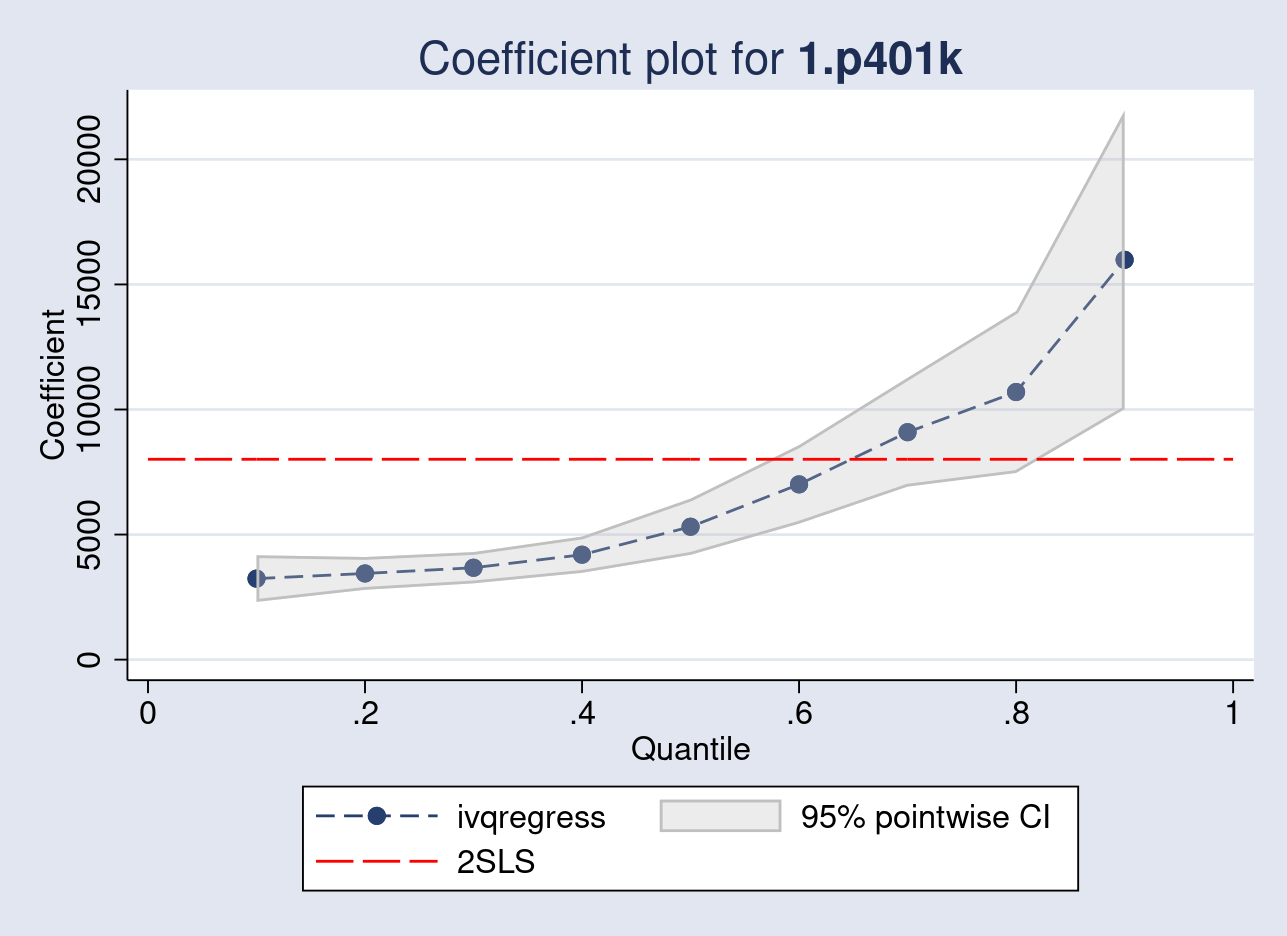
\includegraphics[scale=0.25]{eps/ex3_coefplot1}
\end{figure}

The dots in the plot show the point estimates of {\tt p401k}'s treatment effect
on different conditional quantiles of {\tt asset}, and the grey bound show the
95\% confidence interval.  We see that there is an upward trend of {\tt p401k}'s
treatment effect. At lower level quantiles such as the 10th, 20th, \ldots, 40th
quantiles, the treatment effect is relatively flat.  However, we see the
treatment effect increase significantly in the upper-level quantiles. 

{\tt estat coefplot} is a good way to visualize the treatment effect's trend. If
we want to test some hypotheses regarding the trend and the model statistically,
we can use {\tt estat endogeffects}. For example, we are interested in testing
the following hypotheses.

\begin{itemize} 

\item {\bf No effect}: The 401(k) participation does not affect net financial
asset for all the estimated quantiles; 

\item {\bf Constant effect}: The 401(k) participation's treatment effect is
constant for the different conditional quantiles of asset; 

\item {\bf Dominance}: The 401(k) participation is unambiguously beneficial for
all the estimated quantiles of asset; 

\item {\bf Exogeneity}: The 401(k) participation is exogenous.
\end{itemize}

\clearpage

\begin{stlog}
. estat endogeffects
{\smallskip}
Tests for endogenous effects           Replications = 100
\HLI{17}{\TOPT}\HLI{39}
Null hypothesis  {\VBAR}     KS statistic    95\% Critical value
\HLI{17}{\PLUS}\HLI{39}
No effect        {\VBAR}           11.271                 2.658
Constant effect  {\VBAR}            5.395                 2.650
Dominance        {\VBAR}            0.000                 2.390
Exogeneity       {\VBAR}            4.145                 2.386
\HLI{17}{\BOTT}\HLI{39}
Note: If the KS statistic < critical value, there is
      insufficient evidence to reject the null
      hypothesis.

\end{stlog}

{\tt estat endogeffects} show the Kolmogorov-Smirnov statistic and the 95\%
critical value for each hypothesis. Therefore, we reject the null hypothesis if
the test statistic is greater than the critical value. Otherwise, we can not
reject the null hypothesis.

In particular, we see that the test statistics are greater than the critical
values in testing the hypotheses of no effect, constant effect, and exogeneity.
Thus, with 95\% confidence level, we can reject these three hypotheses. In other
words, we accept the hypotheses that the 401(k) participation has some effect,
treatment is not constant across different quantiles, and 401(k) participation
is endogenous.  In contrast, we can not reject the dominance hypothesis. Thus,
we accept the hypothesis that 401(k) participation is unambiguously beneficial
for all the estimated quantiles of assets.

The test results are consistent with the result of the coefficient plot
produced by {\tt estat coefplot}, where we see that the treatment effects are
positive (dominance and no effect hypotheses) and upward trended (constant
effect hypothesis).

Finally, for reference,  we can also use the SEE estimator to estimate the
model.

\begin{stlog}
. ivqregress smooth assets (i.p401k = i.e401k) income age familysize      ///
>         i.married i.ira i.pension i.ownhome educ, quantile(10(10)90)
{\smallskip}
Fitting smoothed IV quantile regression ...
{\smallskip}
Quantile = .1
Step 1:   bandwidth =  1327.0069    GMM criterion Q(b) =  9.224e-11
Step 2:   bandwidth =  1311.3131    GMM criterion Q(b) =  1.995e-10
{\smallskip}
Quantile = .2
Step 1:   bandwidth =  1272.5204    GMM criterion Q(b) =  2.089e-10
Step 2:   bandwidth =  1237.7195    GMM criterion Q(b) =  3.075e-19
{\smallskip}
Quantile = .3
Step 1:   bandwidth =  1504.4065    GMM criterion Q(b) =  5.407e-13
Step 2:   bandwidth =  1486.4224    GMM criterion Q(b) =  1.136e-10
{\smallskip}
Quantile = .4
Step 1:   bandwidth =  1362.7753    GMM criterion Q(b) =  5.511e-17
Step 2:   bandwidth =  1362.6479    GMM criterion Q(b) =  8.561e-16
{\smallskip}
Quantile = .5
Step 1:   bandwidth =  1302.9736    GMM criterion Q(b) =  2.617e-08
Step 2:   bandwidth =  6079.6881    GMM criterion Q(b) =  2.391e-12
Step 3:   bandwidth =  1438.3068    GMM criterion Q(b) =  8.068e-13
{\smallskip}
Quantile = .6
Step 1:   bandwidth =  1533.5129    GMM criterion Q(b) =  2.679e-18
Step 2:   bandwidth =  1520.1182    GMM criterion Q(b) =  1.141e-19
{\smallskip}
Quantile = .7
Step 1:   bandwidth =  2044.8617    GMM criterion Q(b) =  1.391e-10
Step 2:   bandwidth =  1977.2482    GMM criterion Q(b) =  1.827e-11
{\smallskip}
Quantile = .8
Step 1:   bandwidth =  2503.7256    GMM criterion Q(b) =  3.623e-10
Step 2:   bandwidth =  2458.6714    GMM criterion Q(b) =  2.317e-10
{\smallskip}
Quantile = .9
Step 1:   bandwidth =  3560.2178    GMM criterion Q(b) =  4.301e-12
Step 2:   bandwidth =  3529.3557    GMM criterion Q(b) =  2.932e-10
{\smallskip}
IV quantile regression                                 Number of obs =   9,913
Estimator: Smoothed estimating equations               Wald chi2(81) = 4932.84
                                                       Prob > chi2   =  0.0000
{\smallskip}
\HLI{13}{\TOPT}\HLI{64}
             {\VBAR}               Robust
      assets {\VBAR} Coefficient  std. err.      z    P>|z|     [95\% conf. interval]
\HLI{13}{\PLUS}\HLI{64}
q10          {\VBAR}
     1.p401k {\VBAR}   3191.667   486.2193     6.56   0.000     2238.695    4144.639
      income {\VBAR}   .0318585   .0123707     2.58   0.010     .0076124    .0561046
         age {\VBAR}   128.9268   15.42632     8.36   0.000     98.69178    159.1618
  familysize {\VBAR}  -329.8374   125.4774    -2.63   0.009    -575.7687   -83.90615
             {\VBAR}
     married {\VBAR}
    Married  {\VBAR}  -1480.013   386.4611    -3.83   0.000    -2237.463   -722.5635
             {\VBAR}
         ira {\VBAR}
        Yes  {\VBAR}   7914.049   342.9506    23.08   0.000     7241.878     8586.22
             {\VBAR}
     pension {\VBAR}
Receives ..  {\VBAR}  -5.356704   334.9869    -0.02   0.987     -661.919    651.2056
             {\VBAR}
     ownhome {\VBAR}
        Yes  {\VBAR}   1043.279    308.722     3.38   0.001     438.1945    1648.363
        educ {\VBAR}  -289.8807   53.06713    -5.46   0.000    -393.8904   -185.8711
       _cons {\VBAR}  -7631.313   1214.725    -6.28   0.000    -10012.13   -5250.496
\HLI{13}{\PLUS}\HLI{64}
q20          {\VBAR}
     1.p401k {\VBAR}   3503.744   338.8383    10.34   0.000     2839.633    4167.854
      income {\VBAR}   .0737261   .0084716     8.70   0.000      .057122    .0903302
         age {\VBAR}   114.9688   10.38239    11.07   0.000     94.61965    135.3179
  familysize {\VBAR}  -277.8925   78.67289    -3.53   0.000    -432.0885   -123.6964
             {\VBAR}
     married {\VBAR}
    Married  {\VBAR}  -1160.725   253.6528    -4.58   0.000    -1657.876   -663.5752
             {\VBAR}
         ira {\VBAR}
        Yes  {\VBAR}   8799.905   388.3753    22.66   0.000     8038.703    9561.106
             {\VBAR}
     pension {\VBAR}
Receives ..  {\VBAR}  -33.33779    218.144    -0.15   0.879    -460.8921    394.2165
             {\VBAR}
     ownhome {\VBAR}
        Yes  {\VBAR}   386.2308   201.4194     1.92   0.055    -8.543996    781.0057
        educ {\VBAR}  -194.0516   37.98876    -5.11   0.000    -268.5082    -119.595
       _cons {\VBAR}  -6264.968   792.0489    -7.91   0.000    -7817.356   -4712.581
\HLI{13}{\PLUS}\HLI{64}
q30          {\VBAR}
     1.p401k {\VBAR}   3754.908   320.9631    11.70   0.000     3125.832    4383.984
      income {\VBAR}   .0939826   .0083408    11.27   0.000     .0776348    .1103303
         age {\VBAR}   103.8314   8.712147    11.92   0.000     86.75593    120.9069
  familysize {\VBAR}  -250.4947   59.95479    -4.18   0.000    -368.0039   -132.9855
             {\VBAR}
     married {\VBAR}
    Married  {\VBAR}  -1028.643   217.4311    -4.73   0.000      -1454.8   -602.4861
             {\VBAR}
         ira {\VBAR}
        Yes  {\VBAR}   12008.63   563.5555    21.31   0.000     10904.08    13113.18
             {\VBAR}
     pension {\VBAR}
Receives ..  {\VBAR}  -179.5281   192.0513    -0.93   0.350    -555.9418    196.8855
             {\VBAR}
     ownhome {\VBAR}
        Yes  {\VBAR}   195.7323    162.634     1.20   0.229    -123.0246    514.4891
        educ {\VBAR}  -134.7013    33.4085    -4.03   0.000    -200.1808   -69.22189
       _cons {\VBAR}  -5536.814   637.1917    -8.69   0.000    -6785.686   -4287.941
\HLI{13}{\PLUS}\HLI{64}
q40          {\VBAR}
     1.p401k {\VBAR}   4326.754   371.7419    11.64   0.000     3598.153    5055.354
      income {\VBAR}   .1288469   .0105877    12.17   0.000     .1080955    .1495983
         age {\VBAR}   99.89601   8.289602    12.05   0.000     83.64869    116.1433
  familysize {\VBAR}  -231.3411   53.94265    -4.29   0.000    -337.0668   -125.6155
             {\VBAR}
     married {\VBAR}
    Married  {\VBAR}  -1212.951   216.8328    -5.59   0.000    -1637.935    -787.966
             {\VBAR}
         ira {\VBAR}
        Yes  {\VBAR}   16874.38   801.2841    21.06   0.000     15303.89    18444.86
             {\VBAR}
     pension {\VBAR}
Receives ..  {\VBAR}  -493.1742   198.6221    -2.48   0.013    -882.4663   -103.8821
             {\VBAR}
     ownhome {\VBAR}
        Yes  {\VBAR}   105.4536   152.7777     0.69   0.490    -193.9852    404.8925
        educ {\VBAR}  -114.4753   32.09266    -3.57   0.000    -177.3758   -51.57484
       _cons {\VBAR}  -5216.625   581.4362    -8.97   0.000    -6356.219   -4077.031
\HLI{13}{\PLUS}\HLI{64}
q50          {\VBAR}
     1.p401k {\VBAR}   5364.468   573.3728     9.36   0.000     4240.678    6488.258
      income {\VBAR}   .1679934    .013419    12.52   0.000     .1416925    .1942942
         age {\VBAR}   113.6318   9.352867    12.15   0.000     95.30052    131.9631
  familysize {\VBAR}  -228.7766   57.61072    -3.97   0.000    -341.6916   -115.8617
             {\VBAR}
     married {\VBAR}
    Married  {\VBAR}   -1362.56   238.5988    -5.71   0.000    -1830.205   -894.9153
             {\VBAR}
         ira {\VBAR}
        Yes  {\VBAR}   22402.04   1043.504    21.47   0.000     20356.81    24447.27
             {\VBAR}
     pension {\VBAR}
Receives ..  {\VBAR}   -713.996    220.476    -3.24   0.001    -1146.121   -281.8709
             {\VBAR}
     ownhome {\VBAR}
        Yes  {\VBAR}  -12.71396   161.3703    -0.08   0.937     -328.994    303.5661
        educ {\VBAR}  -102.2889   34.18527    -2.99   0.003    -169.2908   -35.28701
       _cons {\VBAR}  -5672.645   619.7049    -9.15   0.000    -6887.244   -4458.045
\HLI{13}{\PLUS}\HLI{64}
q60          {\VBAR}
     1.p401k {\VBAR}    6964.18   799.1829     8.71   0.000     5397.811     8530.55
      income {\VBAR}   .2422267   .0180009    13.46   0.000     .2069457    .2775078
         age {\VBAR}   145.0532   11.88882    12.20   0.000     121.7515    168.3549
  familysize {\VBAR}  -271.8402   68.28584    -3.98   0.000     -405.678   -138.0024
             {\VBAR}
     married {\VBAR}
    Married  {\VBAR}   -1790.19   278.6729    -6.42   0.000    -2336.379   -1244.001
             {\VBAR}
         ira {\VBAR}
        Yes  {\VBAR}   30029.76   1251.554    23.99   0.000     27576.76    32482.76
             {\VBAR}
     pension {\VBAR}
Receives ..  {\VBAR}  -1063.919   269.4261    -3.95   0.000    -1591.984   -535.8533
             {\VBAR}
     ownhome {\VBAR}
        Yes  {\VBAR}  -79.57029   198.2018    -0.40   0.688    -468.0387    308.8981
        educ {\VBAR}  -128.4236   41.84504    -3.07   0.002    -210.4384   -46.40883
       _cons {\VBAR}  -6708.442   714.0485    -9.39   0.000    -8107.951   -5308.932
\HLI{13}{\PLUS}\HLI{64}
q70          {\VBAR}
     1.p401k {\VBAR}   9002.846   1108.915     8.12   0.000     6829.412    11176.28
      income {\VBAR}   .3555392   .0229067    15.52   0.000      .310643    .4004354
         age {\VBAR}   203.3279   17.59732    11.55   0.000     168.8378     237.818
  familysize {\VBAR}  -314.0023   89.13006    -3.52   0.000     -488.694   -139.3106
             {\VBAR}
     married {\VBAR}
    Married  {\VBAR}  -2396.634   359.7017    -6.66   0.000    -3101.636   -1691.631
             {\VBAR}
         ira {\VBAR}
        Yes  {\VBAR}   38962.04   1621.653    24.03   0.000     35783.66    42140.42
             {\VBAR}
     pension {\VBAR}
Receives ..  {\VBAR}  -1882.868   352.3168    -5.34   0.000    -2573.396    -1192.34
             {\VBAR}
     ownhome {\VBAR}
        Yes  {\VBAR}  -19.74676   271.0796    -0.07   0.942     -551.053    511.5595
        educ {\VBAR}   -163.099   52.90533    -3.08   0.002    -266.7915   -59.40646
       _cons {\VBAR}  -8753.875   954.0692    -9.18   0.000    -10623.82   -6883.934
\HLI{13}{\PLUS}\HLI{64}
q80          {\VBAR}
     1.p401k {\VBAR}   10658.02   1665.467     6.40   0.000     7393.765    13922.27
      income {\VBAR}   .5172628   .0298155    17.35   0.000     .4588255       .5757
         age {\VBAR}   293.9692   24.78395    11.86   0.000     245.3935    342.5448
  familysize {\VBAR}  -407.2737   119.8248    -3.40   0.001    -642.1259   -172.4214
             {\VBAR}
     married {\VBAR}
    Married  {\VBAR}   -3077.77   491.0029    -6.27   0.000    -4040.118   -2115.422
             {\VBAR}
         ira {\VBAR}
        Yes  {\VBAR}   48410.11   2296.042    21.08   0.000     43909.95    52910.27
             {\VBAR}
     pension {\VBAR}
Receives ..  {\VBAR}  -3049.023   515.0161    -5.92   0.000    -4058.436    -2039.61
             {\VBAR}
     ownhome {\VBAR}
        Yes  {\VBAR}   272.4814   412.1642     0.66   0.509    -535.3457    1080.308
        educ {\VBAR}  -131.0776   69.87187    -1.88   0.061    -268.0239    5.868784
       _cons {\VBAR}  -12294.73   1284.692    -9.57   0.000    -14812.68   -9776.781
\HLI{13}{\PLUS}\HLI{64}
q90          {\VBAR}
     1.p401k {\VBAR}   15525.23   3035.965     5.11   0.000     9574.848    21475.61
      income {\VBAR}   .8311508   .0574108    14.48   0.000     .7186277    .9436738
         age {\VBAR}   486.9876   51.61654     9.43   0.000      385.821    588.1541
  familysize {\VBAR}  -586.2617   193.5936    -3.03   0.002    -965.6983   -206.8252
             {\VBAR}
     married {\VBAR}
    Married  {\VBAR}  -3877.165   781.2296    -4.96   0.000    -5408.347   -2345.983
             {\VBAR}
         ira {\VBAR}
        Yes  {\VBAR}   67888.86   4902.106    13.85   0.000     58280.91    77496.81
             {\VBAR}
     pension {\VBAR}
Receives ..  {\VBAR}  -4829.506   898.9147    -5.37   0.000    -6591.346   -3067.665
             {\VBAR}
     ownhome {\VBAR}
        Yes  {\VBAR}   715.6272   722.8727     0.99   0.322    -701.1773    2132.432
        educ {\VBAR}    14.5293   110.8781     0.13   0.896    -202.7878    231.8464
       _cons {\VBAR}  -19953.21   2326.698    -8.58   0.000    -24513.45   -15392.96
\HLI{13}{\BOTT}\HLI{64}
Endogenous: 0b.p401k 1.p401k
 Exogenous: income age familysize 0b.married 1.married 0b.ira 1.ira
            0b.pension 1.pension 0b.ownhome 1.ownhome educ 0b.e401k 1.e401k
{\smallskip}

\end{stlog}

As seen above, after {\tt ivqregress smooth}, we can use {\tt estat coefplot} to
visualize the treatment effect and {\tt estat endogeffects} to test some
hypotheses of particular interest in the context of the IVQR model. To save
space, we will not list the result here.

%------------------------------------------------------------------------------
\subsection{Example 4: Diagnose the IQR estimator}
%------------------------------------------------------------------------------
In this example, we will take a closer look at the IQR estimator and show how to
diagnose the non-convergence issue if it happens. Let us first briefly talk
about the algorithm in the IQR estimator in the context of the 401(k) example.
Intuitively, the IQR estimator can be divided into the following steps.

\begin{enumerate}
\item Define a series of $A = \{\alpha_j\}_{j=1}^J$, where $J$ is the number of
grid points and it can be specified via option {\tt ngrid()}, and $\alpha_j$ is
a candidate solution for the coefficient on {\tt 1.p401k}.

\item For each $\alpha_j$, run the quantile regression of ${\tt asset} - {\tt
1.p401k}*\alpha_j$ on the covariates and some transformations of instruments.
Denote $\gammab_j$ as the coefficients on the instruments and $\Wb_j$ as the
Wald statistic for $\gammab_j$.

\item The IQR solution for $\alpha$ (the coefficients on {\tt 1.p401k}) is the
$\alpha_j$ such that $\gammab_j$ is closest to zero. In other words, the
solution chooses $\alpha_j$ such that the Wald statistic $\Wb_j$ is the
smallest.

\end{enumerate}

We can use {\tt estat waldplot} to visualize the above procedure. Using the
estimation result in Example 1, we first restore the result {\tt est\_iqr} and
then use {\tt estat waldplot} to draw the Wald statistics corresponding to each
grid points.

\begin{stlog}
. estimates restore est_iqr
(results est_iqr are active now)
{\smallskip}
. estat waldplot, name(a)

\end{stlog}

\begin{figure}[H]
\centering
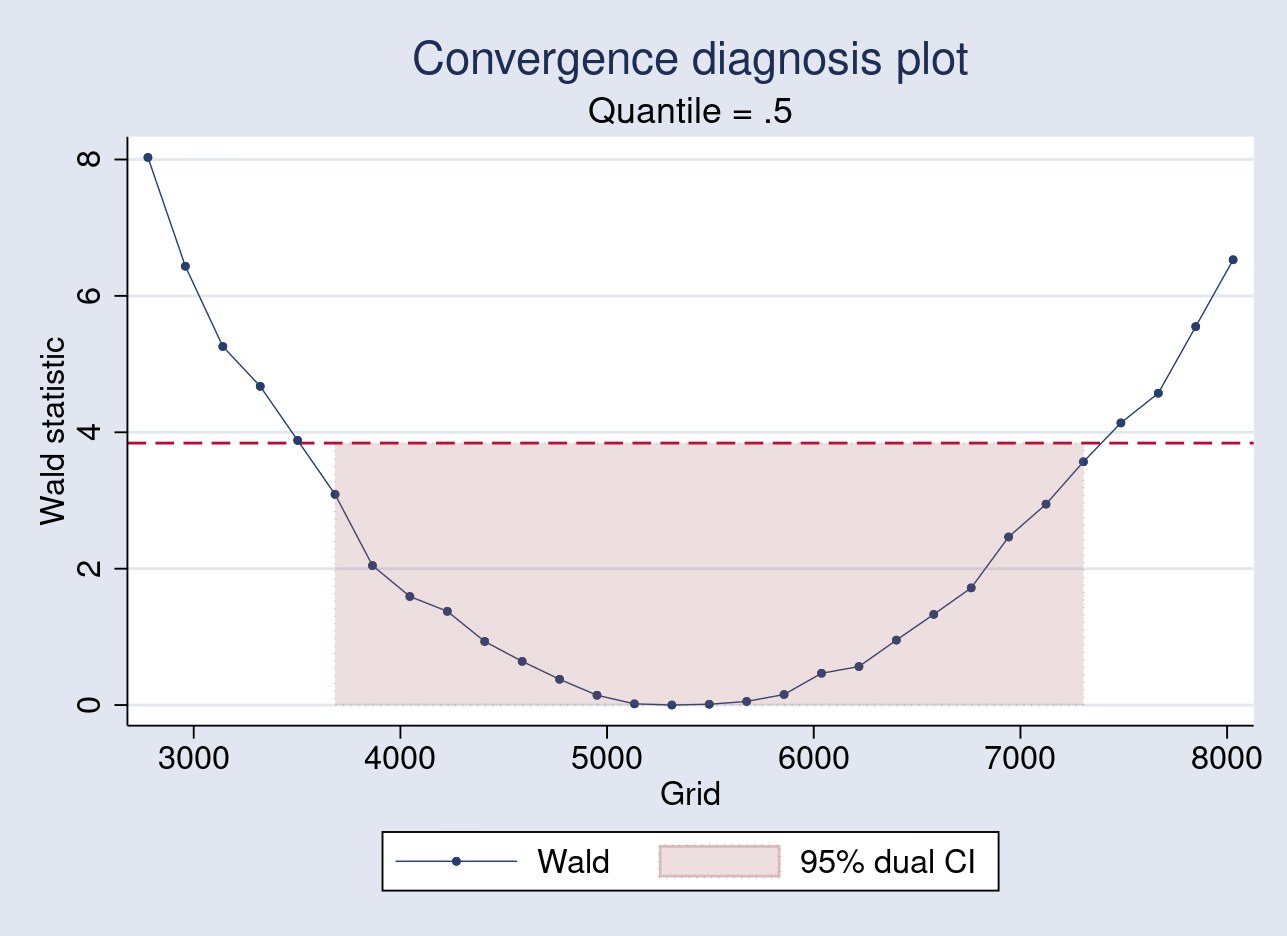
\includegraphics[scale=0.25]{eps/ex4_waldplot1}
\end{figure}

The horizontal axis shows the grid points for $\alpha$, and the vertical axis
shows the values of Wald statistics. Each dot in the plot shows the Wald
statistic corresponding to each grid point. The red dashed line is the 95\%
critical value of the Wald test. Thus, only the Wald statistics below the red
dashed line will not reject the hypothesis that $\gammab_j$ equals zero.
Respectively, the 95\% dual confidence interval is the $\alpha$'s such that the
Wald statistics are below the critical value. See Example 1 for the use of {\tt
estat dualci} to show the numerical values of the dual CI.

By default, {\tt ivqregress iqr} uses the dual CI to generate the lower and
upper bound for the grid points to make sure that the grid covers the true value
of parameter $\alpha$ with a big probability. Sometimes, we may want to
customize the bounds. For example, suppose we want to search grid points between
$3000$ and $6000$. We can use option {\tt bound()} for this purpose.

\begin{stlog}
. cap noi ivqregress iqr assets (i.p401k = i.e401k) income age familysize  ///
>         i.married i.ira i.pension i.ownhome educ, bound(3000 6000)
{\smallskip}
Initial grid
    quantile = 0.50: .........10.........20.........30
{\smallskip}
convergence not achieved
    The grid interval should be wider than the 95\% dual confidence interval.
    Try to set a wider bound using option {\bftt{bound()}}. Use {\bftt{estat waldplot}} for
    diagnosis.

\end{stlog}

We see that {\ivqreg} errors out with ``convergence not achieved". The reason is
that the specified bound is too narrow to cover the true value of the parameter
with a 95\% probability. We can use {\tt estat waldplot} to further visualize
the issue.

\begin{stlog}
. estat waldplot, name(b)

\end{stlog}

\begin{figure}[H]
\centering
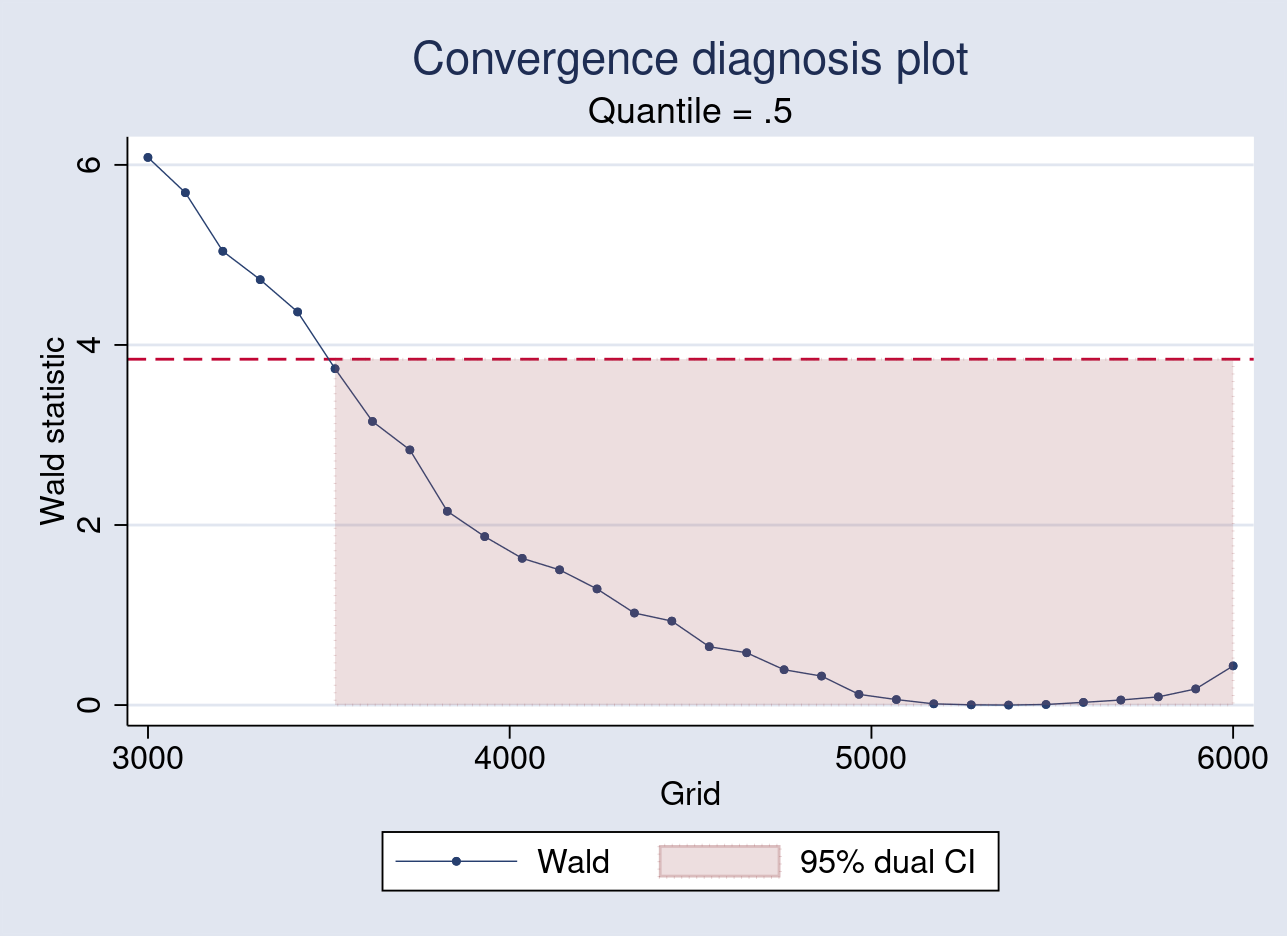
\includegraphics[scale=0.25]{eps/ex4_waldplot2}
\end{figure}

The graph shows that the upper bound $6000$ is too small because we need the
Wald statistics to intersect with the 95\% critical value at both the lower and
upper bound. Now, we can increase the upper bound and see if the IQR estimator
converges. For example, we increase the upper bound to $8000$.

\begin{stlog}
. cap noi ivqregress iqr assets (i.p401k = i.e401k) income age familysize  ///
>         i.married i.ira i.pension i.ownhome educ, bound(3000 8000)
{\smallskip}
Initial grid
    quantile = 0.50: .........10.........20.........30
{\smallskip}
Adaptive grid
    quantile = 0.50: .........10.........20.........30
{\smallskip}
IV median regression                                   Number of obs =   9,913
Estimator: Inverse quantile regression                 Wald chi2(9)  = 1290.41
                                                       Prob > chi2   =  0.0000
{\smallskip}
\HLI{13}{\TOPT}\HLI{64}
             {\VBAR}               Robust
      assets {\VBAR} Coefficient  std. err.      z    P>|z|     [95\% conf. interval]
\HLI{13}{\PLUS}\HLI{64}
     1.p401k {\VBAR}   5332.937   574.5175     9.28   0.000     4206.903    6458.971
      income {\VBAR}    .157381    .012478    12.61   0.000     .1329246    .1818374
         age {\VBAR}   99.78981   8.553978    11.67   0.000     83.02432    116.5553
  familysize {\VBAR}  -199.6165    54.3519    -3.67   0.000    -306.1442   -93.08872
             {\VBAR}
     married {\VBAR}
    Married  {\VBAR}  -1351.309   227.0824    -5.95   0.000    -1796.382   -906.2357
             {\VBAR}
         ira {\VBAR}
        Yes  {\VBAR}   22631.85   1022.023    22.14   0.000     20628.72    24634.98
             {\VBAR}
     pension {\VBAR}
Receives ..  {\VBAR}  -694.1447    210.533    -3.30   0.001    -1106.782   -281.5077
             {\VBAR}
     ownhome {\VBAR}
        Yes  {\VBAR}  -30.67158   154.6947    -0.20   0.843    -333.8676    272.5244
        educ {\VBAR}  -96.30363    32.0715    -3.00   0.003    -159.1626   -33.44465
       _cons {\VBAR}  -4983.758   569.4043    -8.75   0.000     -6099.77   -3867.746
\HLI{13}{\BOTT}\HLI{64}
Endogenous: 0b.p401k 1.p401k
 Exogenous: income age familysize 0b.married 1.married 0b.ira 1.ira
            0b.pension 1.pension 0b.ownhome 1.ownhome educ 0b.e401k 1.e401k
{\smallskip}

\end{stlog}

Now, the IQR estimator converges. We can redraw the Wald plot to confirm that
the proposed grid points interval is indeed wider than the dual confidence
interval.

\begin{stlog}
. estat waldplot, name(c)

\end{stlog}

\begin{figure}[H]
\centering
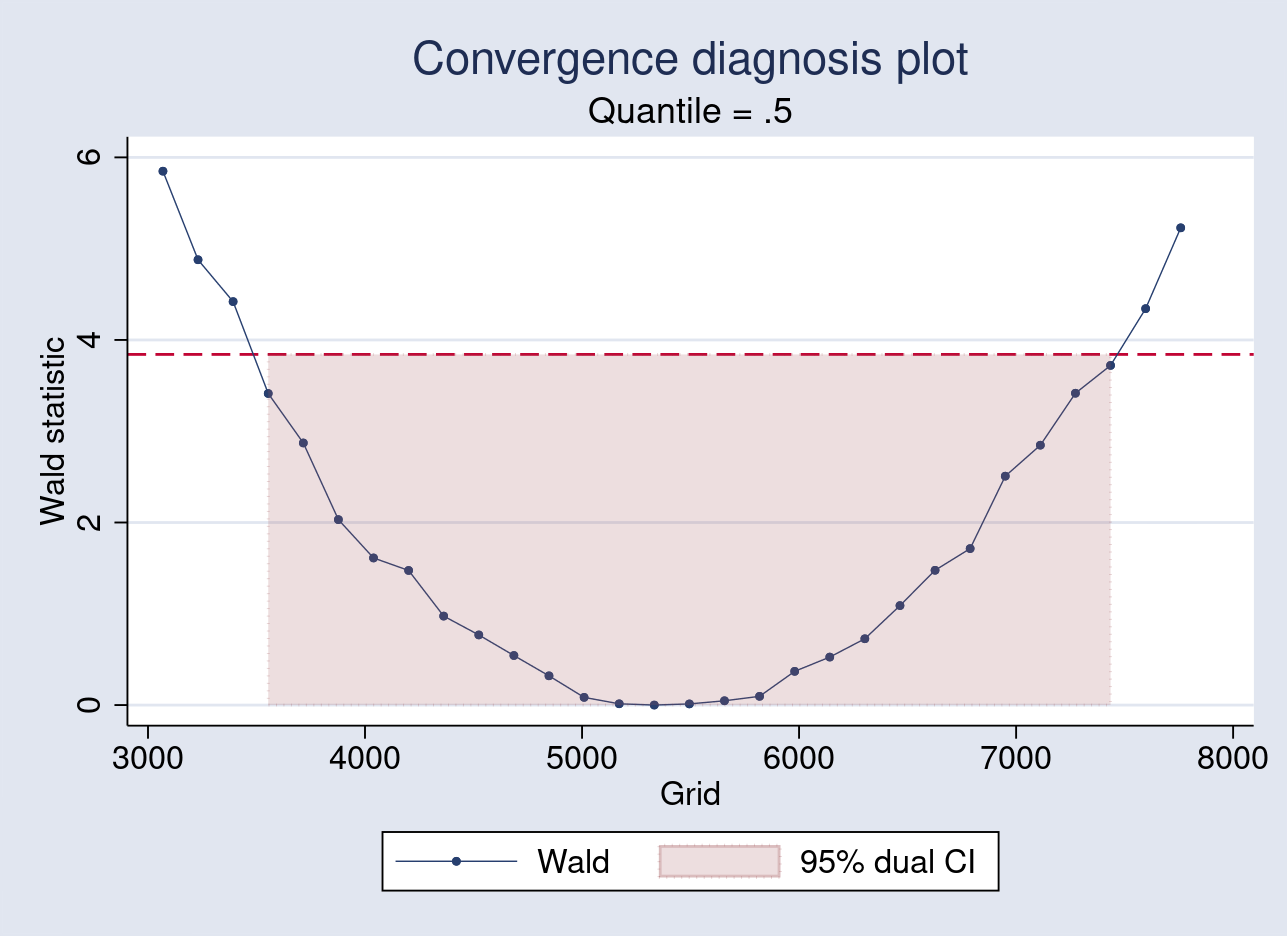
\includegraphics[scale=0.25]{eps/ex4_waldplot3}
\end{figure}

\clearpage

%------------------------------------------------------------------------------
%	Appendix	
%------------------------------------------------------------------------------

% appendix section
\appendix
\section{Appendix}

% proof for the theorem 1
%------------------------------------------------------------------------------
\subsection{Proof for Theorem \ref{th:moment}}	 \label{sec:proof_moment}
%------------------------------------------------------------------------------
\begin{proof}

\begin{align*}
P(Y \leq q(\Db, \Xb, \tau) |\Xb=\xb, \Zb=\zb)
	& \stackrel{(1)}{=} P( q(\Db, \Xb, \UD) \leq q(\Db, \Xb, \tau) |
	\Xb=\xb, \Zb=\zb) \\
	& \stackrel{(2)}{=} P( \UD \leq \tau | \Xb=\xb, \Zb=\zb) \\
	& \stackrel{(3)}{=} \int P(\UD \leq \tau | \Xb=\xb, \Zb=\zb, V=v)
		dP(V=v|\Xb=\xb, \Zb=\zb) \\
	& \stackrel{(4)}{=} \int P(U_{\delta(\xb, \zb, v)} \leq \tau
		| \Xb=\xb, \Zb=\zb, V=v) dP(V=v|\Xb=\xb, \Zb=\zb)  \\
	& \stackrel{(5)}{=} \int P(\Ud \leq \tau
		| \Xb=\xb, \Zb=\zb, V=v) dP(V=v|\Xb=\xb, \Zb=\zb)  \\
	& \stackrel{(6)}{=} P(U_0 \leq \tau | \Xb=\xb, \Zb=\zb) \\
	& \stackrel{(7)}{=} \tau
\end{align*}
Equality (1) by the definition of $Y$ in A5. Equality (2) follows the decreasing
feature of $q()$ in A1. Equality (3) is by the definition of conditional
probability. Equality (4) is by the definition of $\Db$ in A3. Equality (5) holds
because, conditional on $(\Xb, \Zb, v)$, $\Db$ is a constant, and the
distribution of $\Ud$ is identical. Here, we assume $\Db = 0$ in this case.
$\Db$ can be any fixed value in $\mathbbm{D}$. Equality (6) is by definition.
Finally, equality (7) holds because $\Ud \sim U(0,1)$ in A1 and $\Ud$ is
independent of $\Xb$ and $\Zb$ in A2.

\begin{align*}
P(\UD \leq \tau | \Xb=\xb, \Zb=\zb) &= P(U_{\delta(\Xb, \Zb, V)} \leq \tau |\Xb
= \xb, \Zb=\zb) \\
	&= \int P(U_{\delta(\Xb, \Zb, v)}\leq \tau |\Xb=\xb, \Zb=\zb, V=v)
		d P(V=v|\Xb, \Zb)  \\
	&= \int P(U_0 \leq \tau | \Xb=\xb, \Zb=\zb, V=v) d P(V=v | \Xb, \Zb) \\
	&= P(U_0 \leq \tau | \Xb=\xb, \Zb=\zb)
\end{align*}
So conditional on $\Xb$ and $\Zb$, $\UD$ has the same distribution as $\Ud$ for
a fixed value of $\db$.

\end{proof}

From the proof for Theorem \ref{th:moment}, we see that rank similarity
assumption in A4 is the fundamental assumption to convert the conditional
distribution of $\UD$ to $\Ud$ with fixed value $\db$. Here, we discuss the
nuisance underlying this assumption.

First, rank invariance is a particular case of rank similarity. Namely, the
rank invariance assumes $\Ud$ are the same across different values in
$\mathbbm{D}$. While convenient and supported by some applications, the rank
invariance assumption may be too strong in practice.

Second, rank similarity means that given an assignment of treatment, the rank
$\Ud$ is identically distributed. For example, among the individuals who have
$\Xb=\xb$, $\Zb=\zb$, and $D=1$, the distribution of $U_0$ and $U_1$ are the
same. In this formulation, we implicitly assume that one selects the treatment
without knowing the potential outcomes. However, the individuals may know the
distribution of the potential outcomes given $(\Xb, \Zb, v)$ but not the exact
value of $U_0$ for each observation.


% discussion on IQR variance
%------------------------------------------------------------------------------
\subsection{Discussion on Theorem \ref{thm:iqr_var}} \label{sec:discuss_iqrvar}
%------------------------------------------------------------------------------

For a rigorous proof for Theorem \ref{thm:iqr_var}, see \cite{Chernozhukov2006}.
Here I provide a intuitive interpretation. IQR estimator approximately solves
the GMM moment condition in Equation \ref{eq:moment2}, and thus the
variance of IQR estimator can be understood via the GMM approach. We take the
first-order taylor expansion of the sample analog of moment
\ref{eq:moment3} at the true value $\thetab(\cdot)$.  The term,
$\frac{1}{\sqrt{n}} \sum_{i=1}^n l_i(\cdot, \thetab(\cdot))\Psib_i(\cdot)$, is
the moment condition at the true value. The term, $\Jb(\cdot)$ is the gradient of
the moment with respect to $\alphab$ and $\betab$. The term, $\Sb(\tau, \tau')$ is
the variance for the moment
$$
\E \left[ l(\cdot)\Psib(\cdot) l(\cdot)\Psib(\cdot)' \right]
$$
This variance has a block-by-block structure such that the block for the $(\tau,
\tau')$ is $\Sb(\tau, \tau')$.
\begin{align*}
\E &\left[ l(\tau)\Psib(\tau) l(\tau')\Psib(\tau')' \right] \\
 &=  \E \left[ l(\tau) l(\tau')\Psib(\tau)\Psib(\tau')' \right] \\
& = \E\left\{
\E \left[ l(\tau) l(\tau')\Psib(\tau)\Psib(\tau')' |\Xb, \Zb\right]
\right \} \\
& = \E \left \{
\E \left[
l(\tau) l(\tau') | \Xb, \Zb
\right] \Psib(\tau) \Psib(\tau')'
\right \} \\
& = \E \left \{
\E \left[
(\tau - \I (\epsilon(\tau) \leq 0)) (\tau' - \I (\epsilon(\tau') \leq 0)
| \Xb, \Zb
\right] \Psib(\tau) \Psib(\tau')'
\right \} \\
& = \E \left \{
\E \left[
(\tau\tau' - \tau\I (\epsilon(\tau')\leq 0)
- \I(\epsilon(\tau)\leq 0)\tau' + \I (\epsilon(\tau)\leq 0)
\I (\epsilon(\tau') \leq 0)
| \Xb, \Zb
\right] \Psib(\tau) \Psib(\tau')'
\right \}
\intertext{notice that $\E(\I(\epsilon(\tau) \leq 0) = \tau$ by the main
implications in IVQR model in Equation \ref{eq:moment1}. So}
& = \E \left \{
\E \left[
(\tau\tau' - \tau \tau'
- \tau\tau' + \I (\epsilon(\tau)\leq 0) \I (\epsilon(\tau' \leq 0))
| \Xb, \Zb
\right] \Psib(\tau) \Psib(\tau')'
\right \}
\intertext{smaller value of $\tau$ also means greater residuals $\epsilon$, so
$\I (\epsilon(\tau)\leq 0) \I (\epsilon(\tau' \leq 0))$ is simplified to
$\min(\tau, \tau')$}
& = \E \left \{
\E \left[ (\min(\tau, \tau') - \tau\tau')  | \Xb, \Zb \right] 
\Psib(\tau) \Psib(\tau')'
\right \} \\
& =
(\min(\tau, \tau') - \tau\tau') \E \left [ \Psib(\tau) \Psib(\tau')' \right]
\end{align*}

For the gradient, $\Jb(\cdot)$,
\begin{align*}
\Jb(\tau) &= \frac{\partial \E(l(\tau) \Psib(\tau))}{\partial \thetab'} \\
&= \E \left[ \E \left( \frac{\partial
l(\tau) \Psib(\tau)
}{\partial \thetab'} |\Xb, \Db, \Zb \right) \right] \\
&= \E \left[ \E \left( \frac{\partial
l(\tau)
}{\partial \thetab'} |\Xb, \Db, \Zb \right) \Psib(\tau) \right] \\
&= \E \left[  \frac{\partial \E ( l(\tau) |\Xb, \Db, \Zb )
}{\partial \thetab'}  \Psib(\tau) \right] \\
&= \E \left[ \left( \frac{\partial F_{\epsilon}(0 |\Xb, \Db, \Zb)
}{\partial \thetab'}  \right) \Psib(\tau) \right] \\
&= \E \left[f_{\epsilon}(0 |\Xb, \Db, \Zb) \Psib(\tau) [\Db', \Xb'] \right] \\
\end{align*}


% decentralization method
%------------------------------------------------------------------------------
\subsection{Decentralization estimators} \label{sec:dec_method}
%------------------------------------------------------------------------------
One major drawback of the IQR approach is that it suffers from the curse of
dimensionality. When there are more than two endogenous variables, the grid
search computing time becomes slow. Recently, \cite{Kaido2021} proposes to
recast the original problem into finding a Nash equilibrium game solution. The
resulting estimator is called the ``decentralization estimator'' because it
iteratively divides the original problem into small sub-problems, a form of
decentralization. 

Another advantage of the decentralization estimator is that it does not require
choosing extra tuning parameter as in the smoothing GMM approach.

\cite{Kaido2021} proposes three different decentralization algorithms: the
simultaneous contraction-based algorithm, the sequential contraction-based
algorithm, and the root-finding algorithm. The simulations in \cite{Kaido2021}
show that the sequential contraction-based estimator is more stable and faster
than the other two alternatives, so we will only focus on this method.

%------------------------------------------------------------------------------
\subsubsection{Sequential contraction-based algorithm}	
%------------------------------------------------------------------------------
We start by partition the parameter vector $\theta = (\beta', \alpha')'$ into $J
= k_d + 1$ subvectors, where $\theta_1 = \beta$ and $\theta_{j} = \alpha_{j-1}$
for $j = 2, \ldots, J$. Let $\theta_{-j}$ denote all the elements in $\theta$
except $\theta_j$. 

We define the following quantile regression objective functions:

\begin{align}
Q_1 &= \E\left[ \rho_{\tau} \left(Y - X'\theta_1 - 	
	D_1\theta_2 - D_2\theta_3 - \ldots - D_{k_d}\theta_J \right) \right] \\
Q_j &= \E\left[ \rho_{\tau} 
\left(
Y - X'\theta_1 - D_1\theta_2 - D_2\theta_3 - \ldots - D_{k_d}\theta_J 
\right) 
	\frac{Z_{j-1}}{D_{j-1}}
	\right] \qquad \text{for } j=2, \ldots, J 
\end{align}
where $\rho_{\tau}(u) = u(\tau - \I(u < 0))$ is the ``check function''. We
assume that $Z_{j-1}/D_{j-1}$ is well defined and positive. In practice, we can
transform the instruments $Z$ and add a large constant to $D$ to satisfy this
condition.  See Section \ref{sec:reparam} for more discussion.

Suppose there are $J$ players, and each player $j$ has control over $\theta_j$
and take $\theta_{-j}$ as given. The players solve the following optimization
problems:
\begin{align}
	\min_{\tilde{\theta_1}\in R^{k_x}} Q_1(\tilde{\theta_1}, \theta_{-1}) \\
	\min_{\tilde{\theta_j}\in R} Q_j(\tilde{\theta_j}, \theta_{-j}) 
\end{align}
Notice that each problem is just an ordinary weighted quantile regression
problem. 

The solution for $Q_j$ satisfies the first-order condition such that 
\begin{align}
\frac{\partial Q_1}{\partial \theta_1} &= \E\left[ 
	(\tau - \I(
Y - X'\theta_1 - D_1\theta_2 - D_2\theta_3 - \ldots - D_{k_d}\theta_J )
	)X
	\right] = 0 \\
\frac{\partial Q_j}{\partial \theta_j} &= \E\left[ 
	(\tau - \I(
Y - X'\theta_1 - D_1\theta_2 - D_2\theta_3 - \ldots - D_{k_d}\theta_J )
	)Z_{j-1}
	\right] = 0  \qquad j = 2, \ldots, J 
\end{align}
These FOC conditions together form the moment conditions in Equation
(\ref{eq:moment_linear}) implied by the linear IVQREG model. 

Let $L_j(\theta_{-j})$ as the minimizer for $Q_j$. The solution satisfies
$$
	L_j(\theta_{-j}^*) = \theta_j^*
$$
which means $\theta^*$ satisfies the moment condition in Equation
(\ref{eq:moment_linear}) simultaneously. $\theta^*$ is also the Nash equilibrium
of the game.

The sequential contraction-based algorithm is as follows.

%------------------------------------------------------------------------------
\begin{algorithm}[H]\caption{Sequential contraction-based algorithm}
\label{algo:seq}
%------------------------------------------------------------------------------
\begin{enumerate}
	
\item Define the starting value $\theta^{(0)} = (\theta_1^{(0)}, \ldots,
\theta_J^{(0)})$ as the solution of the two-stage-least-square estimator for the
linear IV model.

\item Define the maximum number of iteration K.

\item Define the numerical tolerance level $e_N$.

\item For $k = 1$ to K, do loop
	
\begin{enumerate}
\item $\theta_1^{(k)} = L_1(\theta_{-1}^{(k-1)})$
\item For $j=2, \ldots, J$, do loop
$$
\theta_j^{(k)} = M_j(\theta_{-1}^{(k)}) = L_j
	\left(
	\theta_1^{(k)}, \theta_2^{(k)}, \ldots, \theta_{j-1}^{(k)}, 
	\theta_{\{-1, -2, \ldots, -(j-1)\}}^{(k-1)}
	\right)
$$
\item Compute the relative difference between $\theta_{-1}^{(k)}$ and
$\theta_{-1}^{(k-1)}$, denote it as $\delta$.

\item If $\delta \leq e_N$ or $k > K$, exit the loop.

\end{enumerate}

\item The solution is $\hat{\theta} = (\hat{\theta_1}, \theta_{-1}^{(k)})$, where
$\hat{\theta_1} = L_1(\theta_{-1}^{(k)})$.
\end{enumerate}

\end{algorithm}

\vskip 1cm

To conduct inference, we can employ a regular bootstrap.

\vskip 1cm

%------------------------------------------------------------------------------
\begin{algorithm}[H]\caption{bootstrap the decentralized estimator}
\label{algo:boot}
%------------------------------------------------------------------------------

\begin{enumerate}
\item Using the original sample, estimate $\hat{\theta}$ as in Algorithm
(\ref{algo:seq}).

\item For $b=1, \ldots, B$, do

\begin{enumerate}
\item Draw a bootstrap sample ${W_{i=1}^{N}}^{(b)}$ with replacement.

\item Using ${W_{i=1}^{N}}^{(b)}$ and Algorithm (\ref{algo:seq}), estimate
$\widetilde{\theta^{(b)}}$

\end{enumerate}

\item Let $$
F_B(x) = \frac{1}{B}\sum_{b=1}^B \I(\sqrt{N}(
\widetilde{\theta^{(b)}} - \hat{\theta}) \leq x)
$$
Use $F_B(x)$ as an approximation to the distribution of $\sqrt{N}(\hat{\theta} -
\theta^*)$
\end{enumerate}

\end{algorithm}

%------------------------------------------------------------------------------
\subsubsection{Reparameterization}	
\label{sec:reparam}
%------------------------------------------------------------------------------
The sequential contraction-based algorithm requires that $D_j/Z_j$ is positive
and well defined. Therefore, we need to reparameterize the model to satisfy this
condition.

For the instruments, we can transform $Z_j$ such as 
$$
\tilde{Z_j} = \exp{Z_j}/(1 + \exp{Z_j})
$$
So $\tilde{Z_j}$ will always be positive. Given the original moment condition in
Equation (\ref{eq:moment_linear}) , any transformation of $Z_j$ should also
satisfy this condition.

For the endogenous variable $D_j$, we can add to it a large constant to make the
sum always positive. In particular, suppose $D_j \in (D_{min}, D_{max})$ for
each $j=1, \ldots, k_d$, we add $D_j$ to a constant $c$ such that $c >
|D_{min}|$.  Denote $\tilde{D_j} = D_j + c$.

Suppose the original model is 
$$
	q(D, X, \tau) = \beta_0 + D'\alpha + X'\beta 
$$
After reparameterization, the model becomes
$$
	q(D, X, \tau) = \beta_0 - c \sum_{j=1}^{k_d}\alpha_j 
		+ (D + c)'\alpha + X'\beta 
$$
So the estimated constant is 
$\tilde{\beta_0} = \hat{\beta_0} - c \sum_{j=1}^{k_d}\hat{\alpha_j}$, 
and the estimate for the original constant term
is $ \hat{\beta_0} = \tilde{\beta_0} + c\sum_{j=1}^{k_d}\hat{\alpha_j}$.


%------------------------------------------------------------------------------
\subsubsection{Overidentified case}	
%------------------------------------------------------------------------------
So far, we assume the model is just identified, that is $k_z = k_d$. When there
are more instruments than the endogenous variables, we can use the instrument
$\tilde{D}$, which is the linear projection of $D$ on the space spanned by $Z$
and $X$. Then the objective function in the sequential contraction-based
algorithm becomes:

\begin{align*}
Q_1 &= \E\left[ \rho_{\tau} \left(Y - X'\theta_1 - 	
	D_1\theta_2 - D_2\theta_3 - \ldots - D_{k_d}\theta_J \right) \right] \\
Q_j &= \E\left[ \rho_{\tau} 
\left(
Y - X'\theta_1 - D_1\theta_2 - D_2\theta_3 - \ldots - D_{k_d}\theta_J 
\right) 
	\frac{\widetilde{D_{j-1}}}{D_{j-1}}
	\right] \qquad \text{for } j=2, \ldots, J 
\end{align*}
where $\widetilde{D_{j-1}} = \Psi(\Psi'\Psi)^{-1}\Psi'D_{j-1}$, and $\Psi = (X,
Z)$.

To achieve further efficiency gain, we can use the method in Remark 5 of
\cite{Chernozhukov2006}. In practice, this method also involves
nonparametrically estimating the error term's density function at $0$, which
inevitably requires a choice of the bandwidth. For simplicity, we will not
pursue this path.


%------------------------------------------------------------------------------
%	Bibliography
%------------------------------------------------------------------------------

% reference
\clearpage
\bibliographystyle{sjlatex/sj}
\bibliography{mybib}


\end{document}
